% CVPR 2027 Paper Template; see https://github.com/cvpr-org/author-kit
% [Claude] 2026-10-27: moved to the CVPR 2027 author kit (v1): cvpr.sty, rebuttal.tex and README.md updated; the Paper ID is gone from the template.

\documentclass[10pt,twocolumn,letterpaper]{article}

%%%%%%%%% PAPER TYPE  - PLEASE UPDATE FOR FINAL VERSION
% \usepackage{cvpr}              % To produce the CAMERA-READY version
\usepackage[review]{cvpr}      % To produce the REVIEW version
% \usepackage[pagenumbers]{cvpr} % To force page numbers, e.g. for an arXiv version

% Import additional packages in the preamble file, before hyperref
%% This file contains a number of tweaks that are typically applied to the main document.
%% They are not enabled by default, but can be enabled by uncommenting the relevant lines.


%%
%% Official support for 2-column teaser figure
%%
\usepackage{cuted} %< for strip environment

%%
%% For auto-referencing of figures (see fig/teaser.tex and \label{} therein)
%%
\usepackage{currfile} %< for \currfilebase macro

%%
%% caption and (global) spacing overrides
%%
\usepackage{caption} %< for "\captionof" commands (teaser)
% \setlength{\abovecaptionskip}{.5em} % space above caption
% \setlength{\belowcaptionskip}{1em} % space below caption

%%
%% Packages used by the paper (graphicx, booktabs, amsmath, xcolor, subcaption are loaded by cvpr.sty)
%%
\usepackage{colortbl}      %< \rowcolor in the tables
\usepackage{algorithm}
\usepackage{algpseudocode}

%%
%% Inline annotations; for predefined colors, refer to "dvipsnames" in the xcolor package:
%% https://tinyurl.com/overleaf-colors
%%
\newcommand{\red}[1]{{\color{red}#1}}
\newcommand{\todo}[1]{\textcolor{red}{TODO: #1}}   %< as in the workshop paper
\newcommand{\TODO}[1]{\textbf{\color{red}[TODO: #1]}}
\newcommand{\mynote}[1]{\textcolor{blue}{Note: #1}}
% [Claude] 2026-11-05: per-author tags and a placeholder tag (user request); dvipsnames colours, distinct from the ones above
\newcommand{\placeholder}[1]{\textcolor{Gray}{[Placeholder: #1]}}
\newcommand{\lulu}[1]{\textcolor{ForestGreen}{[Lulu: #1]}}
\newcommand{\lily}[1]{\textcolor{Magenta}{[Lily: #1]}}
\newcommand{\alec}[1]{\textcolor{Cerulean}{[Alec: #1]}}
\definecolor{pink}{HTML}{D9786A}                    %< "MoMo" in the title

%%
%% Content written by Claude (AI assistant). Everything Claude wrote is set in claudecolor and opens with a
%% "[Claude draft]" tag, so it can be reviewed and rewritten before submission:
%%   \claude{...}                              inline text written by Claude
%%   \begin{claudedraft} ... \end{claudedraft}  a block written by Claude (tagged at its start)
%%   \claudenote{...}                          a note from Claude to the authors (not paper text)
%%
\definecolor{claudecolor}{HTML}{6A3D9A}
\newcommand{\claudetag}{\textsf{\scriptsize[Claude draft]}}
\newcommand{\claude}[1]{{\color{claudecolor}#1}}
\newcommand{\claudenote}[1]{{\color{claudecolor}\textsf{\footnotesize[Claude note: #1]}}}
\newenvironment{claudedraft}{\par\color{claudecolor}\noindent\claudetag\ \ignorespaces}{\par}
%%
%% Disable for camera ready / submission by uncommenting these lines:
%%
% \renewcommand{\TODO}[1]{}
% \renewcommand{\todo}[1]{#1}
% \renewcommand{\lulu}[1]{} \renewcommand{\lily}[1]{} \renewcommand{\alec}[1]{}   % [Claude] 2026-11-05: hide the author tags
% \renewcommand{\claudenote}[1]{}
% \renewcommand{\claudetag}{}
% \definecolor{claudecolor}{HTML}{000000}

%%
%% Work harder in optimizing text layout. Typically shrinks text by 1/6 of page, enable
%% it at the very end of the writing process, when you are just above the page limit.
%%
% \usepackage{microtype}

%%
%% Fine-tune paragraph spacing.
%%
% \renewcommand{\paragraph}[1]{\vspace{.5em}\noindent\textbf{#1.}}

%%
%% Globally adjusts space between figure and caption.
%%
% \setlength{\abovecaptionskip}{.5em}

%%
%% Allows "the use of \paper to refer to the project name"
%% with automatic management of space at the end of the word.
%%
% \usepackage{xspace}
% \newcommand{\paper}{ProjectName\xspace}

%%
%% Commonly used math definitions.
%%
% \DeclareMathOperator*{\argmin}{arg\,min}
% \DeclareMathOperator*{\argmax}{arg\,max}

%%
%% Tighten underline.
%%
% \usepackage{soul}
% \setuldepth{foobar}

%%
%% Reconfigure paragraph (tweaks spacing)
%%


% It is strongly recommended to use hyperref, especially for the review version.
% hyperref with option pagebackref eases the reviewers' job.
% Please disable hyperref *only* if you encounter grave issues,
% e.g. with the file validation for the camera-ready version.
%
% If you comment hyperref and then uncomment it, you should delete *.aux before re-running LaTeX.
% (Or just hit 'q' on the first LaTeX run, let it finish, and you should be clear).
\definecolor{cvprblue}{rgb}{0.21,0.49,0.74}
\usepackage[pagebackref,breaklinks,colorlinks,allcolors=cvprblue]{hyperref}

% [Claude] 2026-10-27: the CVPR 2027 template has no Paper ID (removed to avoid leaking IDs); was:
% %%%%%%%%% PAPER ID  - PLEASE UPDATE
% \def\paperID{*****} % *** Enter the Paper ID here
\def\confName{CVPR}
% [Claude] 2026-10-27: 2026 -> 2027
\def\confYear{2027}

%%%%%%%%% TITLE - PLEASE UPDATE
\title{\textcolor{pink}{MoMo}: Incremental \textcolor{pink}{Mo}tion \textcolor{pink}{Mo}deling for Monocular 4D Gaussian Reconstruction}
% Running title of the ECCV version (CVPR has no running head): MoMo: Incremental Motion Modeling

%%%%%%%%% AUTHORS - PLEASE UPDATE
% The review version prints "Anonymous CVPR submission" instead of this block.
\author{Yunze Wei \qquad Lily Goli \qquad Alec Jacobson\\
University of Toronto\\
{\tt\small lulu.wei@mail.utoronto.ca}
}

% [cowrite] Claude co-writing markup. Everything the agent inserts or removes is orange until a human accepts it.
%   \claudeadd{...} inserted text (may hold paragraphs and display math)   \claudedel{...} removed text
%   \begin{claudeblock}...\end{claudeblock} inserted blocks   \claudenote{...} remark for the author
%   \needcite{...} \needref{...} \needimage{...} placeholders for missing citations, references and figures
\usepackage[normalem]{ulem}
\long\def\claudeadd#1{{\color{orange}#1}}
\providecommand{\claudedel}[1]{{\color{orange}\sout{#1}}}
\providecommand{\claudenote}[1]{\textcolor{orange}{\textbf{[Claude: #1]}}}
\providecommand{\needcite}[1]{\textcolor{orange}{[CITE: #1]}}
\providecommand{\needref}[1]{\textcolor{orange}{[NEED REF: #1]}}
\providecommand{\needimage}[1]{\textcolor{orange}{[NEED IMAGE: #1]}}
\newenvironment{claudeblock}{\par\color{orange}}{\par}

\begin{document}
\maketitle

% Sections are in sec/; each section inputs its own figures, tables and algorithms from fig/.
% Commented lines are the parts the workshop version left out.
\begin{abstract}
  4D reconstruction from a single view is highly underconstrained. State-of-the-art methods such as Shape of Motion (SoM) regularize reconstruction using a small set of shared motion bases. \lulu{Do we still want to mention SOM analysis for the final paper?}Yet, we find that test-view quality saturates after only three to five bases, while adding more causes each point to rely on all bases almost equally to explain its motion, severely overfitting the training views. We analyze this behavior across two datasets and propose a progressive optimization scheme that first captures dominant motion and adds new bases only to explain the remaining residual. 

  % Keywords (ECCV only; CVPR has no keyword field): Novel View Synthesis, 4D Reconstruction
\end{abstract}

\section{Introduction and Background}
\label{sec:intro}
% zoom in quickly on the problem (4D from monocular video is needed (e.g. robotics ~cite jitendra), but underconstrained problem, to solve one SoTA method is SoM where having a few basis motion regularize the solution)

% dig a hole (the problem with SoM type methods: the regularization of motion comes from having a small number of motion basis but we analyze and see more than 5 doesnt help with test views, and therefore having more than 5 just leads to equal usage of all bases while all bases severely overfitting to training views)

% fill the hole (We first extensively analyze this problem over two datasets and show with different number of basis the test PSNR doesnt improve after 5 basis. We then propose a different optimization scheme where we make sure that the first few bases fit the low frequency (major) parts of the motion while the new basis is added only to fit the remaining residual motion. We show quant and qual results on iphone dataset where we improve over SoM by X db in PSNR on the test views.)
Recovering dynamic 3D scenes matters for downstream applications like learning robotic behavior from human demonstrations~\cite{paliwal2026dexterous}, autonomous driving\cite{}, video content generation\cite{}, and virtual reality~\cite{}.  
The problem has been initially addressed using NeRF based reconstruction methods\cite{}, and more recently using 3DGS\cite{}and feedforward 4D models. In the multi-view setup, the input data are multiple videos at different camera views. However, in reality, casually captured videos often only have access to a single camera view, leading to the underconstrained monocular reconstruction problem. Many recent methods address the lack of regularization in a single camera view by representing the scene with 3D Gaussians~\cite{kerbl20233d} and optimizing their motion per video using preprocessed depth, camera, flow, and track priors~\cite{lei2025mosca, wang2025shape, stearns2024dynamic, wang2025gflow}. 
Methods fall into several paradigms such as per-Gaussian motion parameters~\cite{stearns2024dynamic, wang2025gflow}, deformation fields that map canonical Gaussians to each frame~\TODO{Deformable 3dgs yang et all, 4DGS Wu et al}, sparse control points or motion graphs to which the Gaussians are skinned~\cite{huang2024sc, lei2025mosca}, and motion bases shared by all Gaussians~\cite{kratimenos2024dynmf, wang2025shape, liang2025himor}. \TODO{dynMF}
One widely used idea, popularized by Shape of Motion (SoM)~\cite{wang2025shape}, is to represent the scene with 3D Gaussians and regularize their motion through a small set of shared motion bases.
A separate line of work trains feedforward models that regress 4D Gaussians directly, without per-video optimization~\cite{lin2026movies}, trading generality for speed.

Despite their success at being able to reconstruct the training video, previous methods show severe overfitting to training views, causing extreme visual distortions in where the novel view camera is far away from the position of the training camera. We find that Shape of Motion's motion bases regularization is only effective with a surprisingly small number. Across the DyCheck \cite{gao2022dynamic}and NVIDIA \cite{yoon2020novel}datasets, test-view quality saturates after roughly three to five bases. Adding more bases does not improve test-view reconstruction; instead, the basis coefficients become increasingly uniform, with each Gaussian relying similarly on many bases to explain its motion, leading to increased overfitting of the training views. This also leads to a large number of redundant parameters that, in fact, hurt novel view synthesis quality.

To solve these problems, we propose MoMo, an incremental optimization scheme for motion modelling, in which the initial bases capture the dominant, low-frequency motion, while additional bases are introduced to explain the remaining residual.
Our process solely operates on the preprocessing stage of initializing motion bases, providing a more regularized and interpretable bases allocation to model the rigid bodies in a scene. Our contributions are two-fold: 

\begin{itemize}
\item{We propose MoMo, an incremental motion modelling method that identifies dominant motions of 3D tracks.}
\item{Our method allows for efficient 4DGS reconstruction that uses fewer parameters compared to other State-of-the-art methods while being better or on par in terms of PSNR and other reconstruction metrics.} 
\end{itemize}






% --------- original Lulu's version ------------
% Reconstruction of dynamic motion from monocular videos has important applications in video understanding, robotics, and virtual reality. 
% One common approach in recent computer vision has been to represent the scene using 3D Gaussian Splatting (3DGS)~\cite{kerbl20233d}, and modelling the movement of these Gaussians through time~\cite{wang2025shape, wang2025gflow, huang2024sc}.
% Among these methods, the 3D Gaussian parameters (mean, covariance, color, opacity) are typically defined in a single frame then moved temporally using a per-frame deformation. 
% The granularity of this deformation ranges drastically, from per Gaussian parameters on the scale of $10^5$~\cite{stearns2024dynamic}, deformation fields with $10^3$ control points~\cite{lei2025mosca}, to compact representing using only around 10 bases trajectories~\cite{wang2025shape, kratimenos2024dynmf}.

% In this paper, we demonstrate that novel view synthesis quality saturated at a surprisingly low number of bases trajectories (2-5), and further additions only improve training views. 
% To solve this problem, we propose a method for adaptively clustering motion guided by the photometric reconstruction gradient, such that reconstruction quality is increased without harming the coarse rigid body motions in the scene.
% [Claude] 2026-11-05: sections 2, 3 and 6, the acknowledgements and the supplementary switched back on (user request); were commented out.
\section{Related Work}

\lulu{lulu to write}

\label{sec:related-work}
% [Claude] 2026-11-05: three subsections (user request); the feedforward paragraph moved up under its own heading.
\subsection{Dynamic Scene Reconstruction}
Many recent methods address the lack of regularization in a single camera view by representing the scene with 3D Gaussians~\cite{kerbl20233d} and optimizing their motion per video using pretrained depth, camera, flow, and track priors~\cite{lei2025mosca, wang2025shape, stearns2024dynamic, wang2025gflow}.

\subsection{Feedforward Reconstruction}
A separate line of work trains feedforward models that regress 4D Gaussians directly, without per-video optimization~\cite{lin2026movies}, trading generality for speed.

\subsection{Motion Bases Representation}
Shape of Motion (SoM)~\cite{wang2025shape} models scene motion with a small set of shared $B$ SE(3) \textit{motion bases} $\mathbf{T}^{(b)}_{0 \to t}$ that varies with time; at time $t$ the center $\mu_t^g$ and rotation $R_t^g$ of Gaussian $g$ is computed as a weighted sum of these bases, relative to a canonical frame $t_0$ chosen as the frame with the most visible tracks. The blending weights $w^{(b)}_g$, which are constant in time, define each Gaussian's association to each basis, and are optimized per-Gaussian alongside the bases themselves. SoM finds $B=10$ bases sufficient, outperforming per-Gaussian SE(3) motion. We show that only a few bases improve novel view synthesis, while more bases help only the training views reconstruction.


%------- original version ------
% \textbf{4D Monocular Reconstruction} 
% Recent works use 3DGS~\cite{kerbl20233d} for rendering dynamic scenes for its efficiency and quality. 
% 3D motion from the scene is optimized using supervision pretrained models for depth, camera, and dense track prediction to infer 3D geometry from the limited single 2D view.

% A recent state-of-the-art method, Shape-of-Motion~\cite{wang2025shape}, represents the scene motion as a set of SE(3) \textit{motion bases} $\mathbf{T}^{(b)}_{0 \to t} = \begin{bmatrix} \mathbf{R}^{(b)}_{0 \to t} & \mathbf{t}^{(b)}_{0 \to t} \end{bmatrix}$ that act upon Gaussian mean $\mu_t$ and rotation $\mathbf{R}_t$. 
% A canonical frame $t_0$ is picked as the frame with the most visible tracks, and the mean and rotation of each Gaussian is obtained using a linear combination of the bases.

% % \begin{equation}
% %     \mathbf{T}_{0 \to t} = \sum_{b=0}^{B} \mathbf{w}^{(b)} \mathbf{T}_{0 \to t}^{(b)}.
% %     \label{eq:motion-basis}
% % \end{equation}

% In the paper,~\cite{wang2025shape} claims that a very small number of bases is enough to reconstruct the scene and uses B=10 bases for all experiments.
% Furthermore, ablation studies claim that performance degrades when motion is modelled per-Gaussian SE(3) rather than as a linear combination of bases.
% We provide an analysis and show that only the few bases lead to an improvement in novel view synthesis quality, while further increasing the bases counts only lead to improvement in training but not novel views.


\section{Analysis of Number of Bases}

We conduct a hyperparameter sweep over the number of bases $\mathbf{B}$ from 1-20 per scene for the SoM baseline to analyze its behaviour as more distinct transforms are used to model the scene.
We track training/test PSNR as $B$ increases and examine how Gaussian basis blending weights are distributed across bases, on the benchmarks DyCheck~\cite{gao2022dynamic} dataset and NVIDIA dataset~\cite{yoon2020novel}~\ref{fig:sweep-avg}. 
Fig.~\ref{fig:basis-psnr} shows test PSNR saturates as early as 3 bases while training PSNR keeps rising, indicating overfitting rather than better motion modeling.

% Was an inline wrapfigure in sec/4_method.tex (workshop version); caption = its commented-out caption.
\begin{figure}[t]
  \centering
  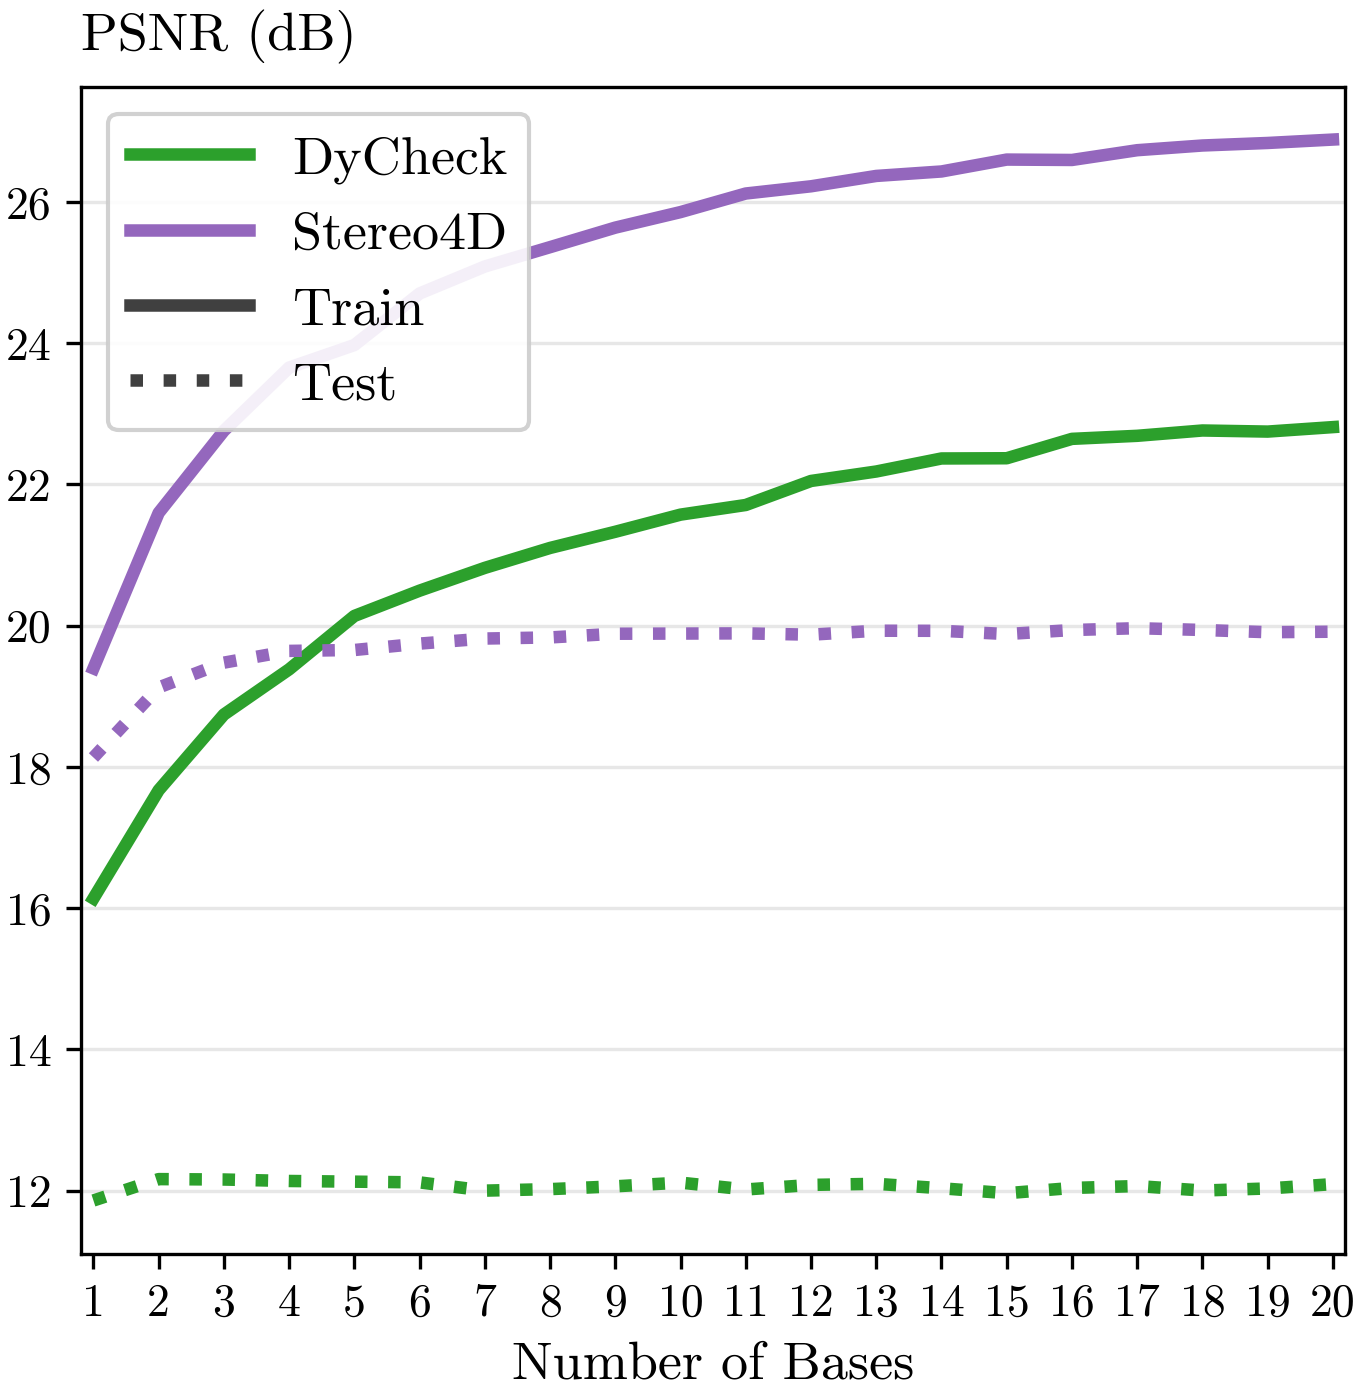
\includegraphics[width=0.75\linewidth]{img/combined-sweep.png}
  \caption{Training PSNR rises with more bases, while test PSNR quickly saturates. \lulu{Replace with NVIDIA instead of stereo}}
  \label{fig:basis-psnr}
\end{figure}


% % Was a commented-out wrapfigure in sec/4_method.tex (workshop version); caption = its commented-out caption.
% Label renamed from fig:basis-utilization, which fig/synthetic_weights.tex uses.
\begin{figure}[t]
  \centering
  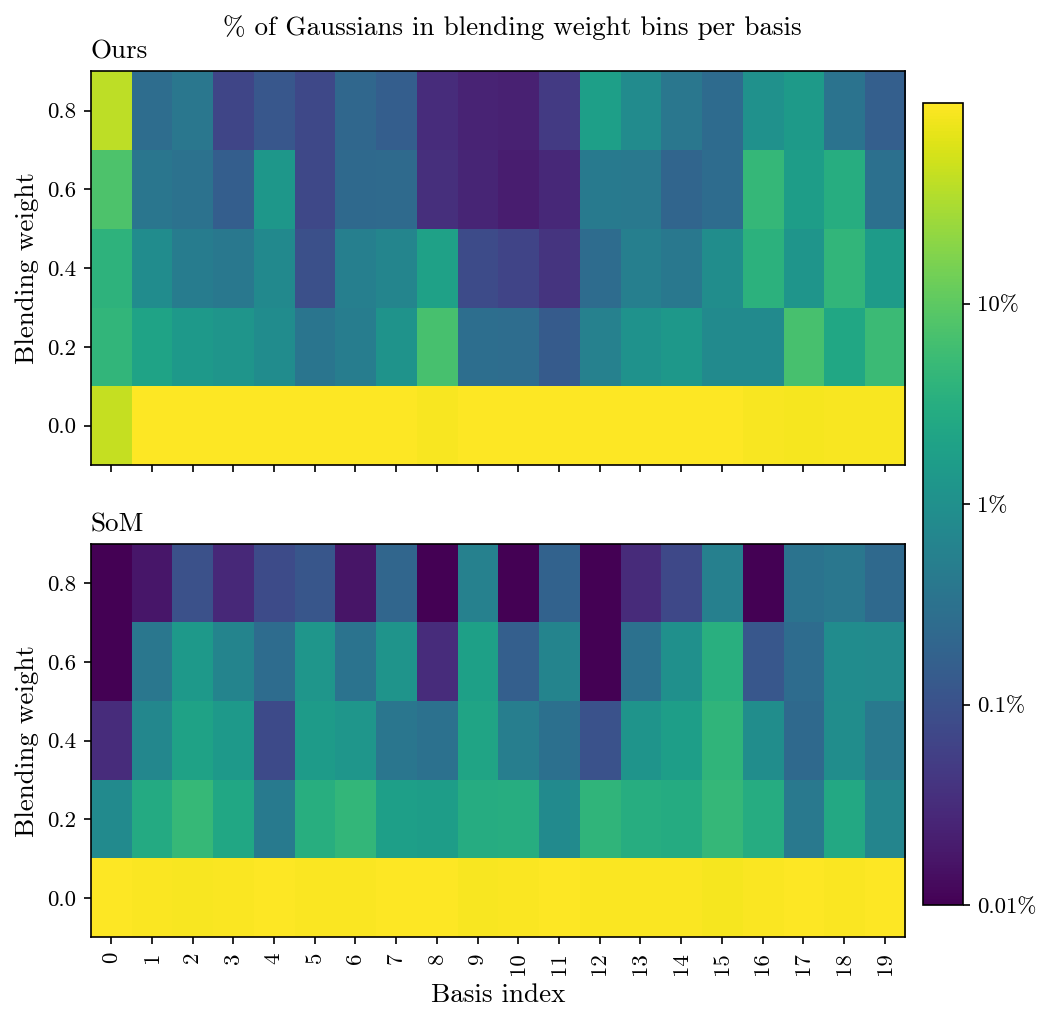
\includegraphics[width=\linewidth]{img/heatmap.png}
  \caption{Average Gaussian basis blending weights across bases.}
  \label{fig:basis-utilization-heatmap}
\end{figure}


In addition to standard benchmarks, we construct a synthetic pinwheel scene with two motion modes: a dominant rotation about the center and a localized translation of the blade tips, affecting roughly $20\%$ of the tracks. The inset compares the average blending weight assigned to each basis after fitting SoM. With 20 bases, SoM assigns substantial, nearly uniform weight across many bases, failing to reflect the underlying two-mode structure. The additional capacity is instead used to minimize the training-view photometric loss, producing noisy, overfit trajectories. This suggests that increasing the number of bases weakens the regularization provided by the compact 3--5 basis model. As a preview of our approach, the weighting profile shown in the inset instead concentrates motion in a few bases, while reserving other bases for smaller residual motions. We formalize this idea through the incremental optimization scheme introduced in the next section.


\section{Method}
\label{sec:method}

% \begin{figure*}[t]
  \centering
  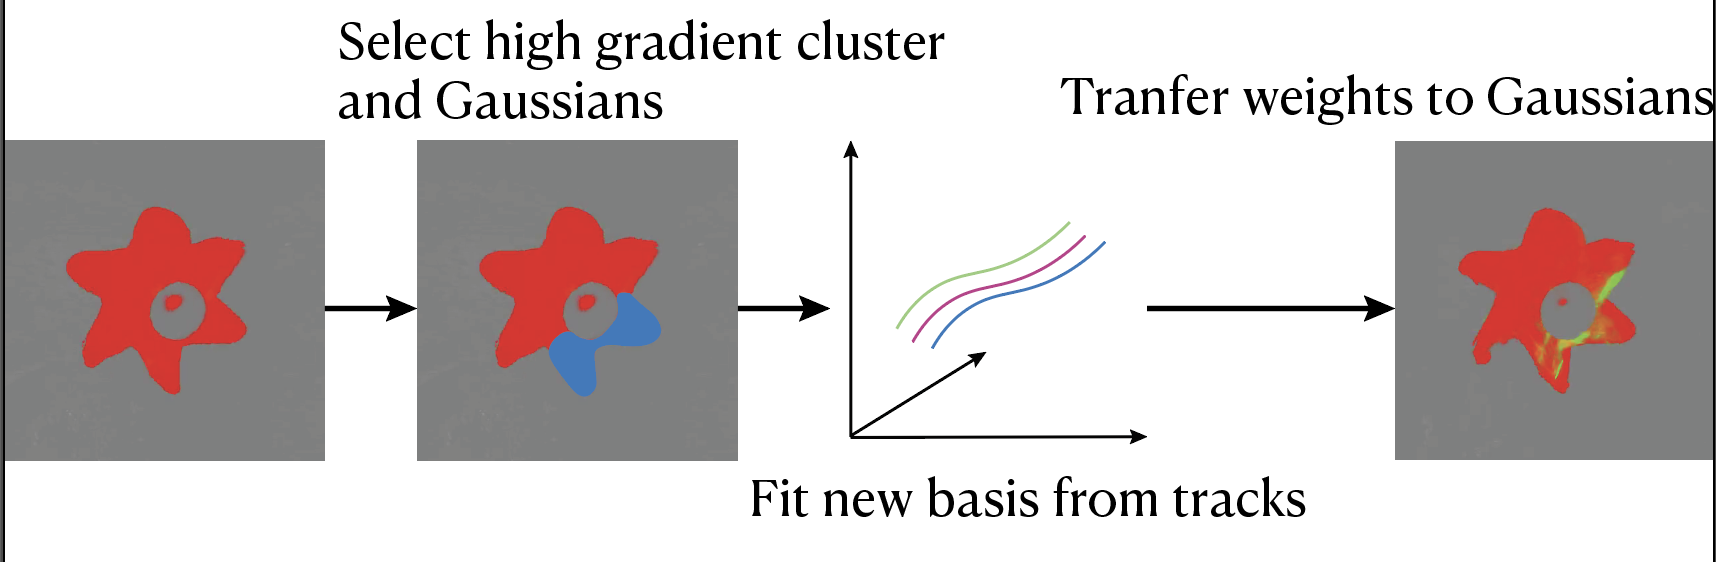
\includegraphics[width=\linewidth]{img/pipeline-draft.png}
  \caption{Overview of our adaptive motion basis densification pipeline.}
  \label{fig:pipeline}
\end{figure*}

\begin{figure*}[t]
  \centering
  \setlength{\tabcolsep}{1pt}
  \begin{tabular}{@{}c@{\hspace{2pt}}ccccc@{}}
    \rotatebox{90}{\makebox[0.247\linewidth][c]{\footnotesize Apple}} &
      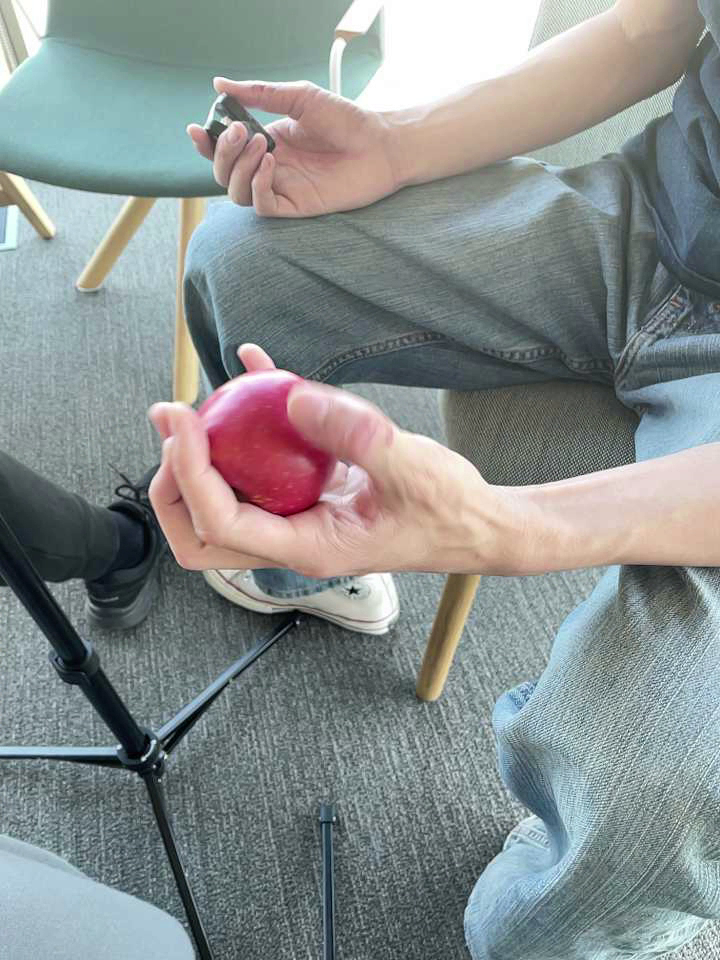
\includegraphics[width=0.185\linewidth]{img/comparison/apple_gt.png} &
      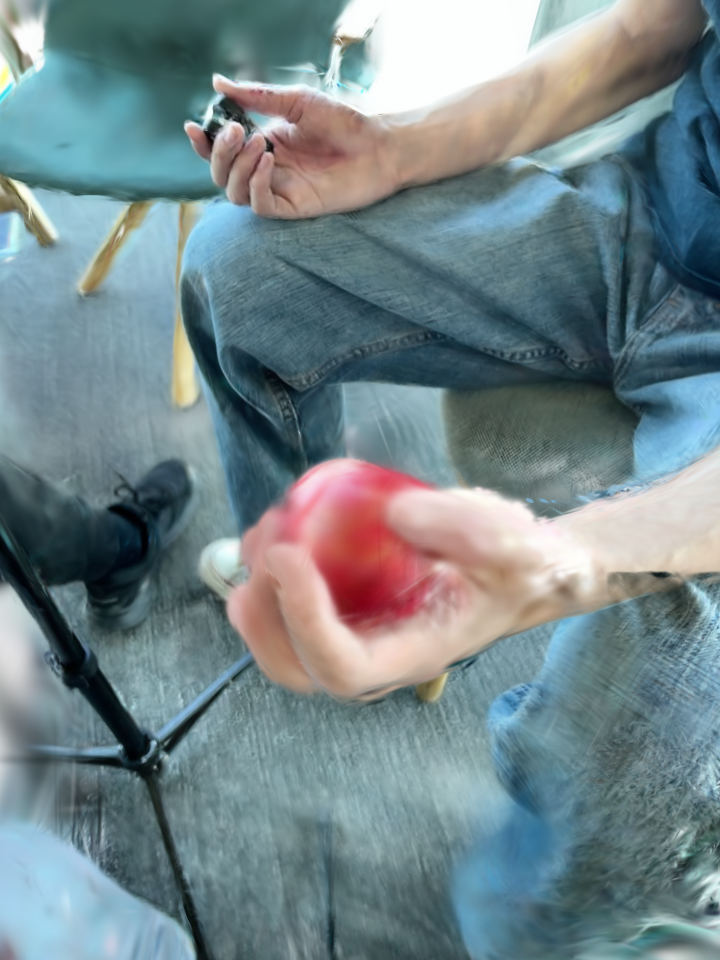
\includegraphics[width=0.185\linewidth]{img/comparison/apple_ours.png} &
      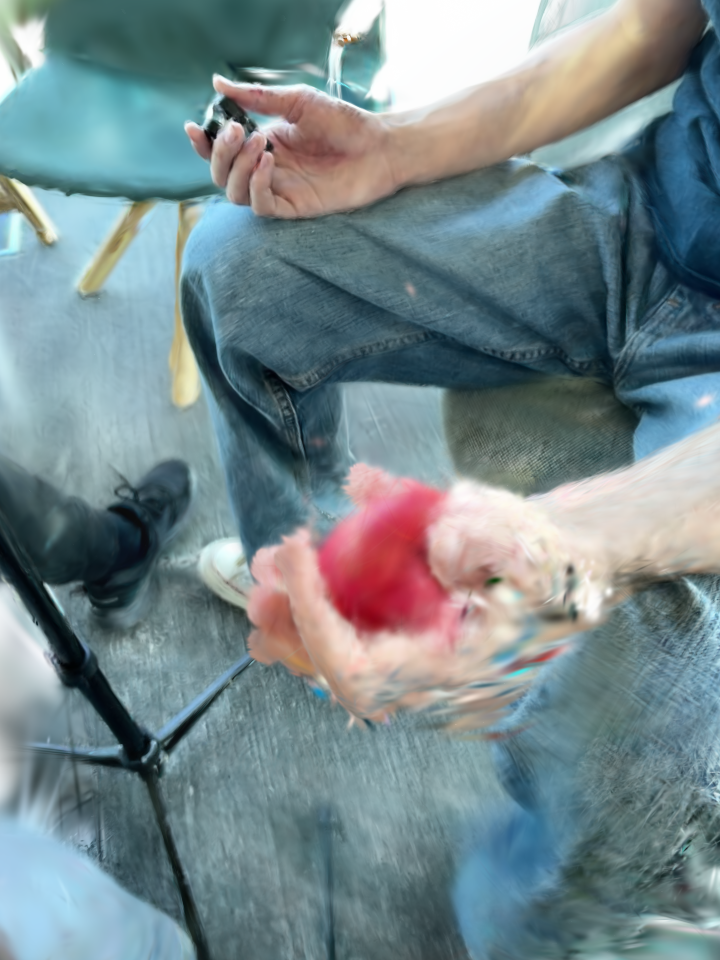
\includegraphics[width=0.185\linewidth]{img/comparison/apple_som.png} &
      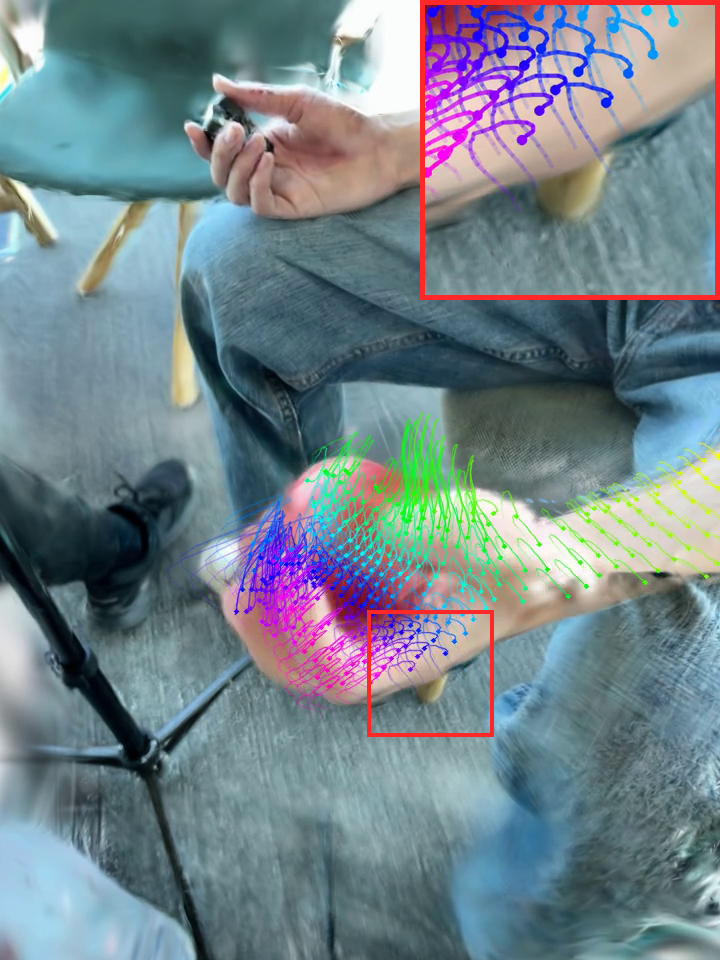
\includegraphics[width=0.185\linewidth]{img/comparison/apple_ours_tracks.png} &
      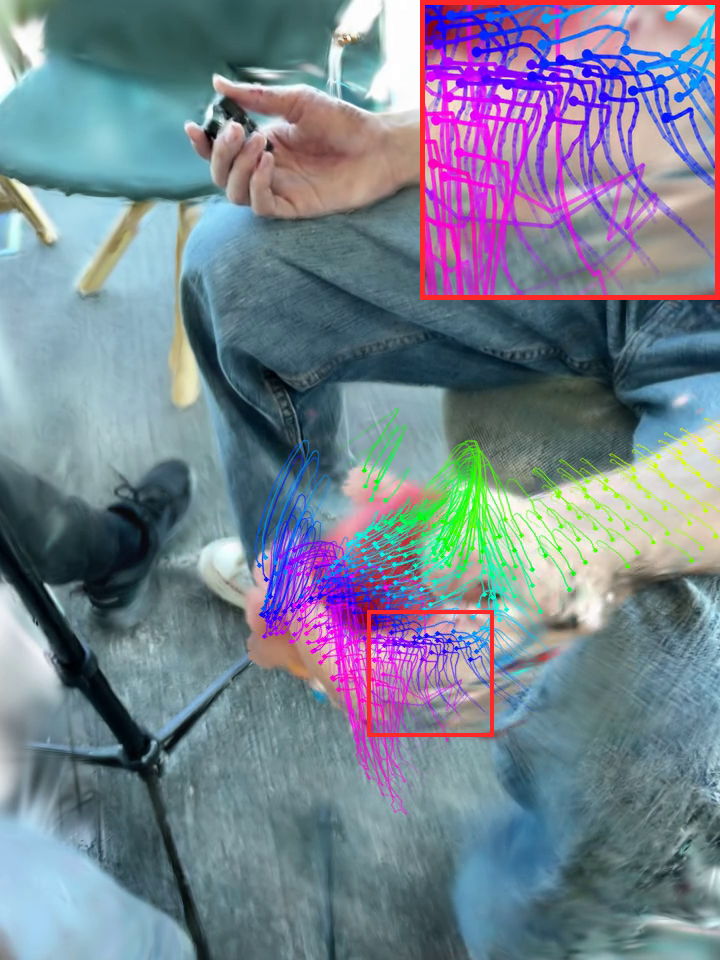
\includegraphics[width=0.185\linewidth]{img/comparison/apple_som_tracks.png} \\
    \rotatebox{90}{\makebox[0.247\linewidth][c]{\footnotesize Paper Windmill}} &
      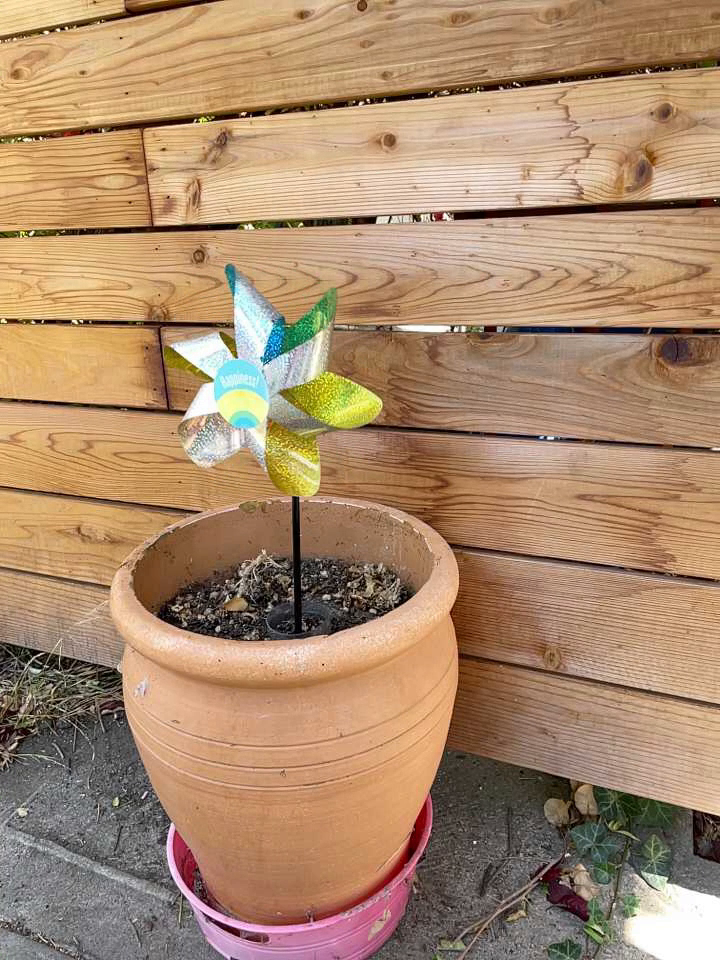
\includegraphics[width=0.185\linewidth]{img/comparison/windmill_gt.png} &
      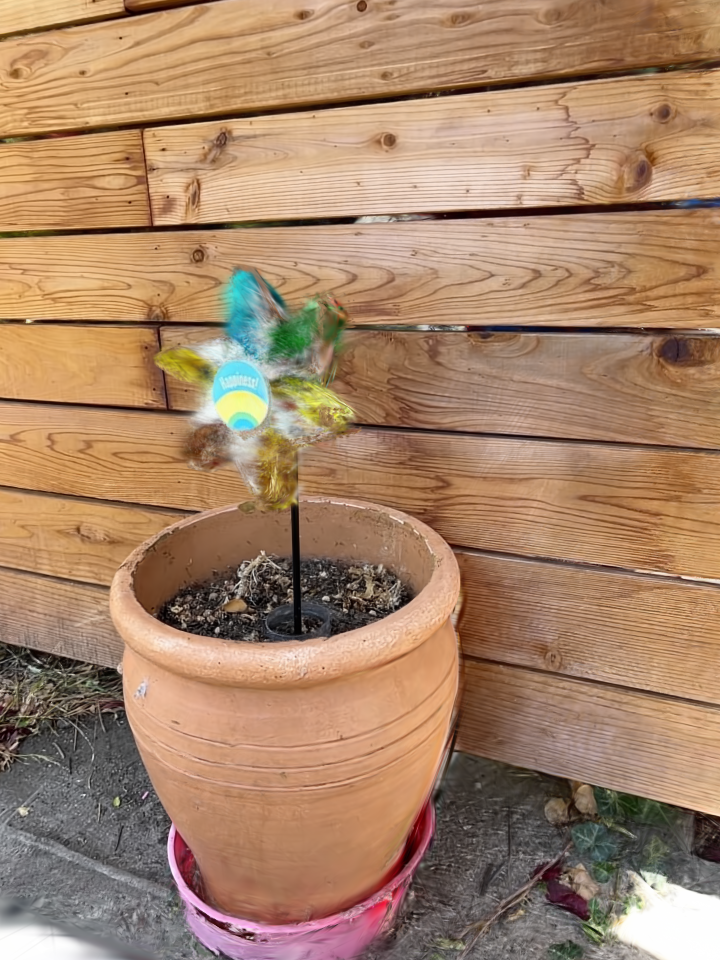
\includegraphics[width=0.185\linewidth]{img/comparison/windmill_ours.png} &
      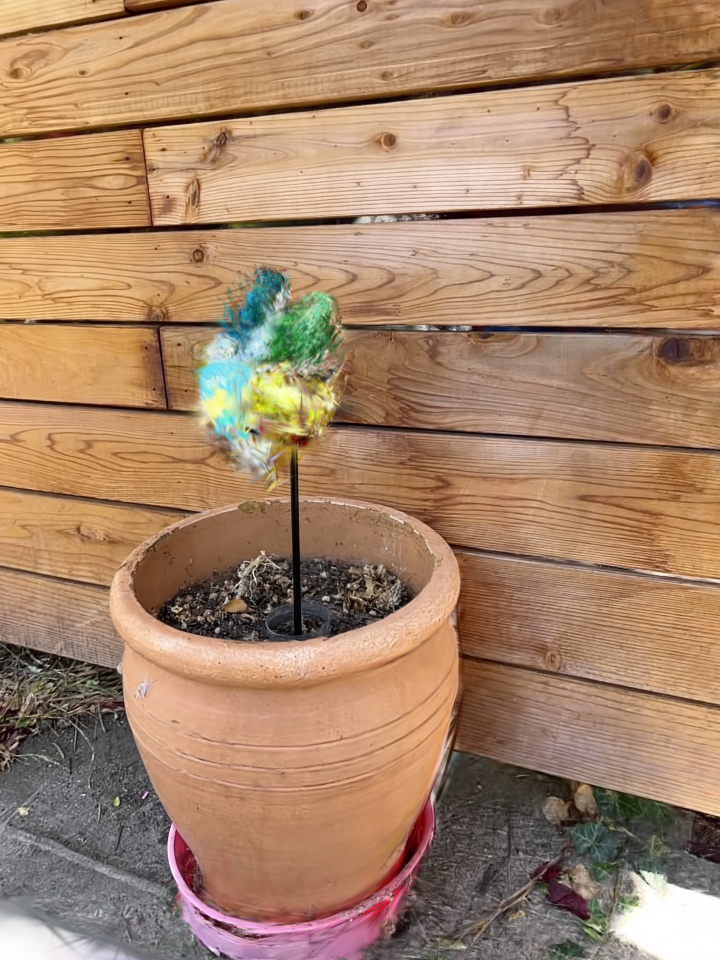
\includegraphics[width=0.185\linewidth]{img/comparison/windmill_som.png} &
      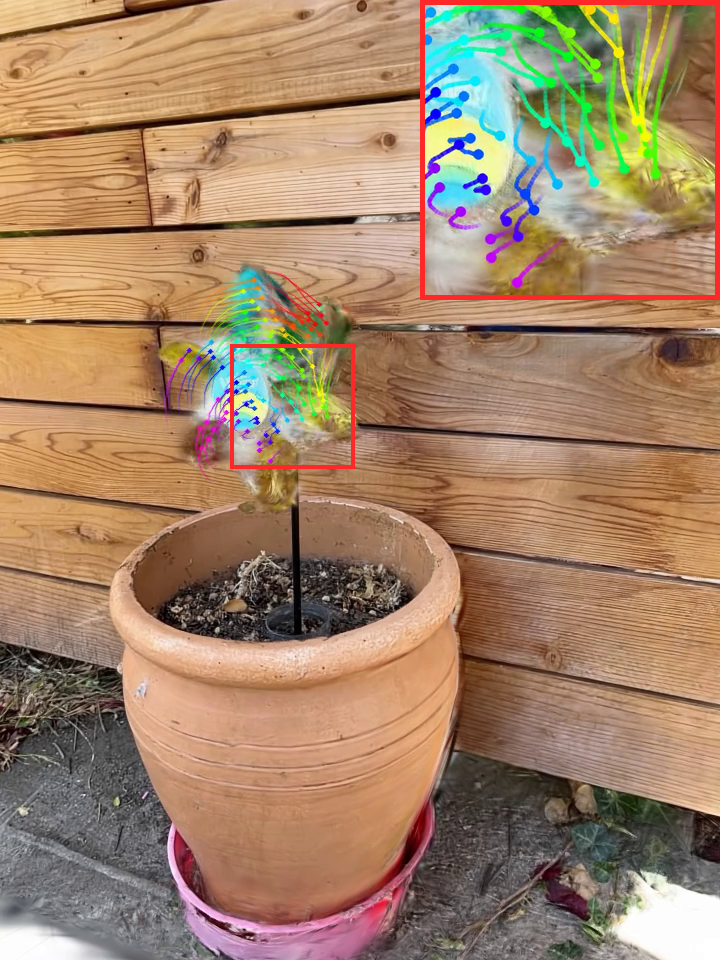
\includegraphics[width=0.185\linewidth]{img/comparison/windmill_ours_tracks.png} &
      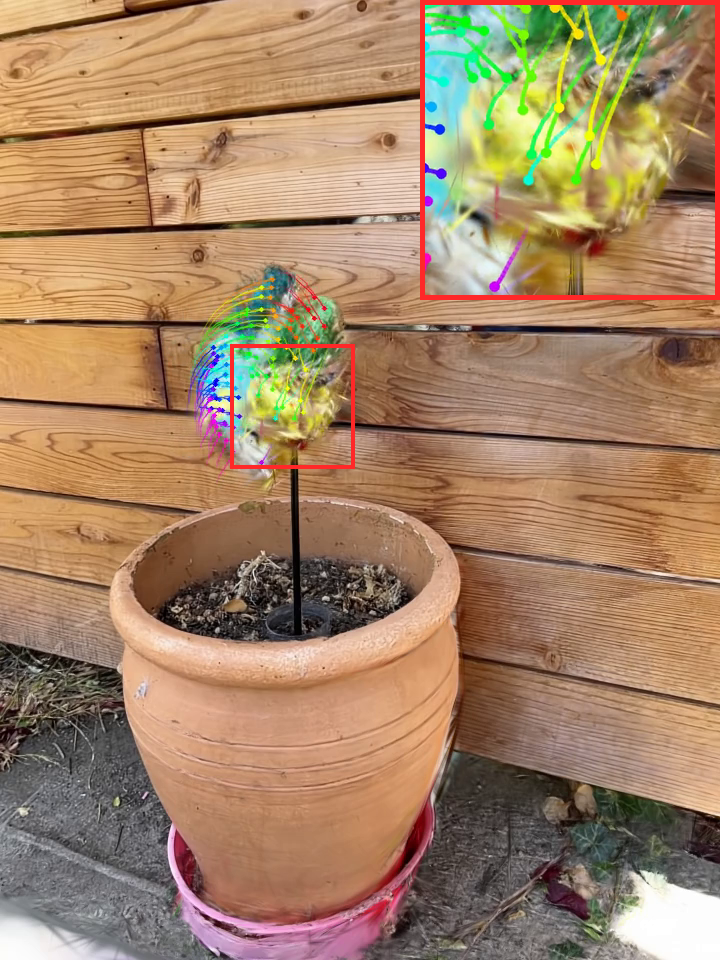
\includegraphics[width=0.185\linewidth]{img/comparison/windmill_som_tracks.png} \\
    
     & \makebox[0.185\linewidth][c]{\footnotesize GT (Test View)} &
       \makebox[0.185\linewidth][c]{\footnotesize Ours} &
       \makebox[0.185\linewidth][c]{\footnotesize SoM} &
       \makebox[0.185\linewidth][c]{\footnotesize Ours (Tracks)} &
       \makebox[0.185\linewidth][c]{\footnotesize SoM (Tracks)} \\
  \end{tabular}
 \caption{\lulu{Replace with updated visualizations + all the baselines}Our method retains regularization toward the main motion modes, while SoM overfits and degrades on the test view.}
  \label{fig:qualitative-comparison}
\end{figure*}
  % results figure (two columns): input here so it lands before the references
% [Claude] 2026-11-05: the per-scene tables moved to the supplementary, sec/X_suppl.tex (user request).
% % Claude, generated by tests/candidate_full_tables.py --fmt tex --ds iPhone --ours split_init --partial (branch momo-modes; ours = MoMo = L2 + clustering + 5 % cutoff, no children; block B 10, user 2026-11-04); orange = not yet accepted.
\begin{table*}[t]
  \centering
  \footnotesize
  \setlength{\tabcolsep}{4pt}
  \begin{tabular}{@{}lcccccccccc@{}}
    \toprule
     & & \multicolumn{3}{c}{PSNR\,$\uparrow$} & \multicolumn{3}{c}{SSIM\,$\uparrow$} & \multicolumn{3}{c}{LPIPS\,$\downarrow$} \\
    \cmidrule(lr){3-5} \cmidrule(lr){6-8} \cmidrule(l){9-11}
    Scene & $B$ & SoM-10 & SoM-$B$ & Ours & SoM-10 & SoM-$B$ & Ours & SoM-10 & SoM-$B$ & Ours \\
    \midrule
    apple & 5 & \textbf{16.38} & 16.28 & 16.36 & 0.744 & 0.744 & \textbf{0.747} & 0.525 & 0.525 & \textbf{0.518} \\
    teddy & 8 & 13.94 & 14.06 & \textbf{14.09} & 0.558 & 0.561 & \textbf{0.562} & 0.509 & 0.512 & \textbf{0.506} \\
    spin & 9 & \textbf{17.27} & 17.14 & 17.10 & \textbf{0.697} & 0.696 & 0.695 & 0.294 & 0.296 & \textbf{0.292} \\
    paper-windmill & 9 & 19.55 & \textbf{19.57} & 19.55 & \textbf{0.553} & \textbf{0.553} & 0.552 & 0.200 & \textbf{0.198} & 0.200 \\
    block & 10 & \textbf{16.93} & \textbf{16.93} & 16.83 & \textbf{0.638} & \textbf{0.638} & \textbf{0.638} & \textbf{0.417} & \textbf{0.417} & 0.418 \\
    \midrule
    Average & 8.2 & \textbf{16.81} & 16.79 & 16.79 & 0.638 & 0.638 & \textbf{0.639} & 0.389 & 0.390 & \textbf{0.387} \\
    \bottomrule
  \end{tabular}
  \caption{\claudetag\ Metrics on the covisible pixels (the dataset's covisibility masks, as in DyCheck) on the held-out views of DyCheck (iPhone)~\cite{gao2022dynamic}, per scene: ours
    (\cref{sec:split-init}) against SoM~\cite{wang2025shape} with its default 10 bases (SoM-10) and with as many bases
    as ours (SoM-$B$). $B$: number of bases of our method, chosen by its $\tau = 0.05$ cutoff. Mean over three seeds; last row: average over the scenes.
    Best value in bold. }
  \label{tab:full-dycheck}
\end{table*}
  % results tables (two columns), same reason
% % Claude, generated by tests/candidate_full_tables.py --fmt tex --ds NVIDIA --ours split_init --partial (branch momo-modes; ours = L2 + clustering, no children); orange = not yet accepted.
% Claude 2026-11-05: Umbrella at the 5 % rule's B = 6 (all three seeds; ours + SoM-6 trained on Killarney, outputs/bdf_killarney,
% linked into outputs/bdf), so every row is at the rule's B. Rows other than Umbrella and Average unchanged by the regeneration.
\begin{table*}[t]
  \centering
  \footnotesize
  \setlength{\tabcolsep}{4pt}
  \begin{tabular}{@{}lcccccccccc@{}}
    \toprule
     & & \multicolumn{3}{c}{PSNR\,$\uparrow$} & \multicolumn{3}{c}{SSIM\,$\uparrow$} & \multicolumn{3}{c}{LPIPS\,$\downarrow$} \\
    \cmidrule(lr){3-5} \cmidrule(lr){6-8} \cmidrule(l){9-11}
    Scene & $B$ & SoM-10 & SoM-$B$ & Ours & SoM-10 & SoM-$B$ & Ours & SoM-10 & SoM-$B$ & Ours \\
    \midrule
    Balloon1 & 4 & \textbf{23.89} & \textbf{23.89} & 23.86 & 0.793 & \textbf{0.794} & 0.792 & \textbf{0.058} & 0.059 & 0.060 \\
    Balloon2 & 6 & \textbf{23.97} & 23.91 & 23.93 & \textbf{0.831} & 0.830 & \textbf{0.831} & \textbf{0.073} & 0.074 & 0.074 \\
    Jumping & 8 & \textbf{20.22} & 20.19 & 20.11 & \textbf{0.701} & 0.700 & 0.696 & \textbf{0.143} & 0.145 & 0.150 \\
    Playground & 7 & \textbf{17.03} & 17.01 & 17.00 & \textbf{0.553} & \textbf{0.553} & \textbf{0.553} & \textbf{0.158} & 0.162 & 0.162 \\
    Skating & 5 & \textbf{27.87} & 27.81 & 27.75 & \textbf{0.914} & \textbf{0.914} & 0.912 & \textbf{0.048} & 0.049 & 0.050 \\
    Truck & 6 & 27.56 & 27.58 & \textbf{27.76} & 0.876 & 0.877 & \textbf{0.878} & 0.052 & 0.052 & \textbf{0.049} \\
    Umbrella & 6 & 23.23 & 23.22 & \textbf{23.25} & \textbf{0.572} & \textbf{0.572} & 0.571 & \textbf{0.168} & \textbf{0.168} & 0.170 \\
    \midrule
    Average & 6.0 & \textbf{23.40} & 23.37 & 23.38 & \textbf{0.749} & 0.748 & 0.748 & \textbf{0.100} & 0.101 & 0.102 \\
    \bottomrule
  \end{tabular}
  \caption{\claudetag\ Metrics on the covisible pixels (the dataset's covisibility masks, as in DyCheck) on the held-out views of NVIDIA Dynamic Scenes~\cite{yoon2020novel}, per scene: ours
    (\cref{sec:split-init}) against SoM~\cite{wang2025shape} with its default 10 bases . $B$: number of bases of our method, chosen by its $\tau = 0.05$ cutoff. Mean over three seeds; last row: average over the scenes.
    Best value in bold. }
  \label{tab:full-nvidia}
\end{table*}


% [Claude] 2026-11-05: preliminaries subsection drafted (user request).
\subsection{Preliminaries: 3D Gaussian Splatting}
\label{sec:prelim}
3D Gaussian Splatting (3DGS)~\cite{kerbl20233d} represents a scene as a set of anisotropic 3D Gaussians.
Each Gaussian $g$ has a center $\boldsymbol{\mu}_g$, a rotation $\mathbf{R}_g$ and per-axis scales $\mathbf{s}_g$, which give its covariance $\boldsymbol{\Sigma}_g = \mathbf{R}_g \operatorname{diag}(\mathbf{s}_g)^2 \mathbf{R}_g^\top$, as well as an opacity $o_g$ and a color $\mathbf{c}_g$.
A view is rendered by projecting the Gaussians onto the image plane, sorting them by depth and alpha-compositing them front to back,
\begin{equation}
  \mathbf{C}(\mathbf{p}) = \sum_{i} \mathbf{c}_i\, \alpha_i \prod_{j<i} (1 - \alpha_j) ,
  \label{eq:3dgs}
\end{equation}
where $\alpha_i$ is the opacity $o_i$ times the projected 2D Gaussian of $i$ evaluated at pixel $\mathbf{p}$.
Since the rasterization is differentiable, all parameters are optimized with a photometric loss on the input images.
For a dynamic scene, SoM~\cite{wang2025shape} defines the Gaussians in a canonical frame $t_0$ and moves their centers and rotations over time (\cref{sec:split-init}).

% [Claude] 2026-11-05: "Motion Bases Analysis" moved to sec/3_analysis.tex as 3.2 (user request); here its heading and figure inputs are commented out and its text is struck.
% \subsection{Motion Bases Analysis}
% % Was an inline wrapfigure in sec/4_method.tex (workshop version); caption = its commented-out caption.
\begin{figure}[t]
  \centering
  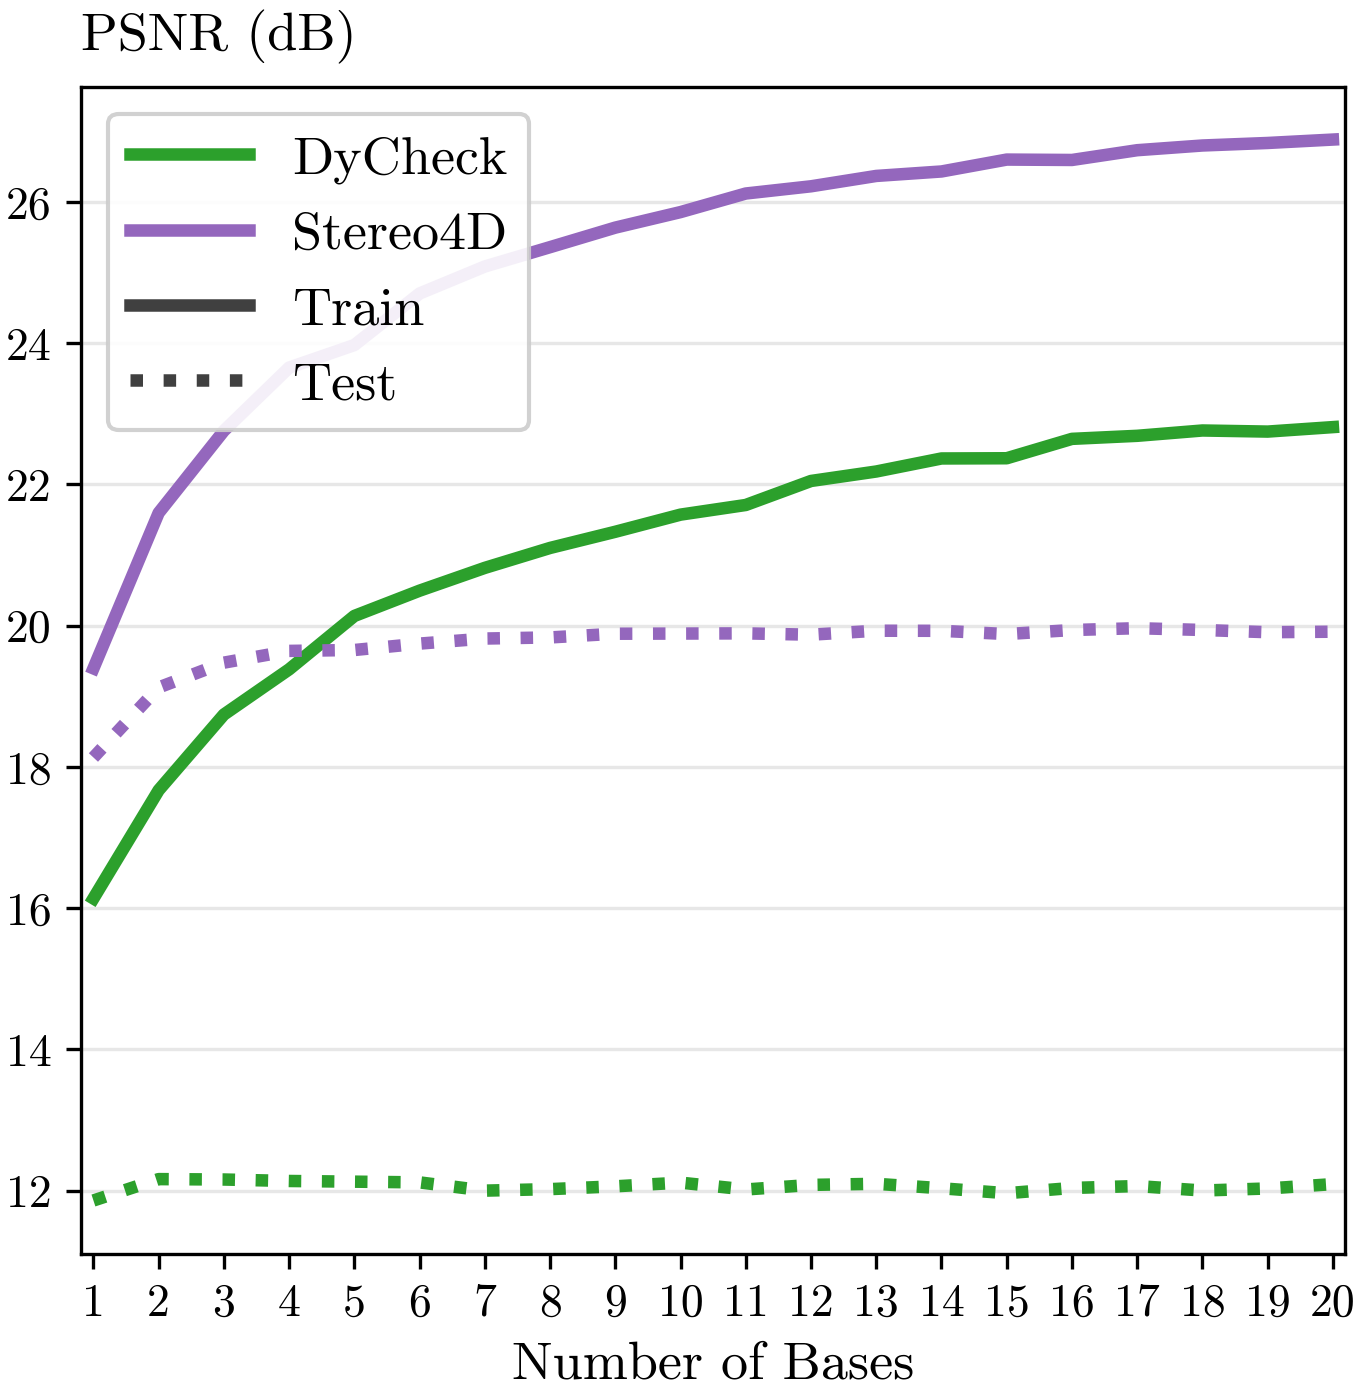
\includegraphics[width=0.75\linewidth]{img/combined-sweep.png}
  \caption{Training PSNR rises with more bases, while test PSNR quickly saturates. \lulu{Replace with NVIDIA instead of stereo}}
  \label{fig:basis-psnr}
\end{figure}

%The Stereo4D dataset presents an easier benchmark due to the high overlap between the training and validation views.

% % Was a commented-out wrapfigure in sec/4_method.tex (workshop version); caption = its commented-out caption.
% Label renamed from fig:basis-utilization, which fig/synthetic_weights.tex uses.
\begin{figure}[t]
  \centering
  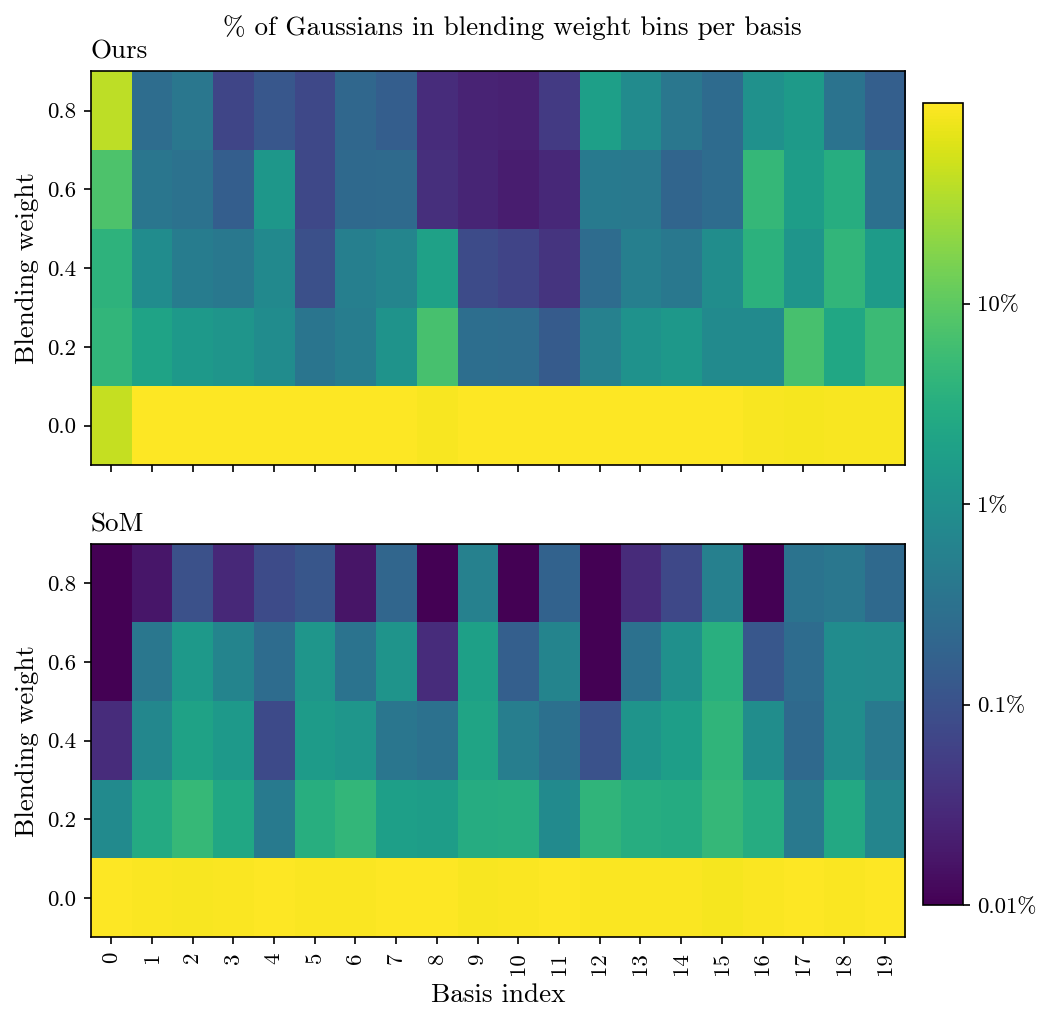
\includegraphics[width=\linewidth]{img/heatmap.png}
  \caption{Average Gaussian basis blending weights across bases.}
  \label{fig:basis-utilization-heatmap}
\end{figure}



%\subsection{Progressive Motion Addition}

%Motivated by this, we replace the fixed basis count $B$ with an adaptive scheme that grows bases where the motion model fails, using the photometric loss gradient as a densification signal, inspired by 3DGS densification~\cite{kerbl20233d}. We start by initializing only a single basis, following the initialization scheme in SoM~\cite{wang2025shape} using precomputed TAPIR~\cite{doersch2023tapir} tracks. Then optimize one basis at a time, freezing previously added bases so each new basis refines local motion without disturbing motion already captured.

%For each Gaussian $g$ with blending weight $w_g^{(b)}$ for basis $b$ and center $\mu_g$, we define its \textit{error contribution} to that basis as $e_g^{(b)} = w_g^{(b)} \lVert \partial \mathcal{L}_{\mathrm{RGB}} / \partial \mu_g \rVert_2^2$. Every few iterations, we compute the basis-level error $e^{(b)} = \sum_g e_g^{(b)} / \sum_g w_g^{(b)}$, the normalized sum of error contributions over all Gaussians, and flag $b$ for densification if $e^{(b)} > \tau$ ($\tau=10^{-5}$). Within a flagged basis, we take the top $15\%$ of Gaussians by error contribution and match each to its nearest TAPIR track in the canonical frame. A new basis is pre-trained on these tracks alone, with all other parameters frozen, using a per-track L2 loss weighted by TAPIR's confidence and visibility scores. We then unfreeze all motion and appearance parameters and jointly optimize against the photometric loss for 1500 steps until the next basis densification.

% ------ original version -------
% Rather than setting the number of motion bases B as a predetermined hyperparameter, our method instead grows the bases adaptively using the photometric loss gradient as a densification signal, inspired by the control steps in 3DGS~\cite{kerbl20233d}.
% We segment the moving part of the input video using SAM2~\cite{ravi2024sam2} and initialize with one cluster using KMeans clustering on track velocity and initialize the motion basis with Procrustes.
% This first transform represents the average motion of all tracks in the scene.

% After the initialization, We optimize one new basis at a time and freeze all previously added bases, so that each new basis refines local motion without disrupting the global rigid motion captured by earlier bases.
% This setup allows more transforms to be fitted to regions of complex motions dynamically and for the number of bases required to be tailored for each scene.

% \textbf{Notation.}
% Let $N$ be the number of foreground moving Gaussians, with optimizable parameters $(\mu_0, R_0, s, o, c)$.
% For the current set of $B$ active bases, let $w_g^{(b)}\!\in\![0,1]$ be the post-softmax coefficient of Gaussian $g$ on basis $b$.
% We write $t_0$ for the canonical frame, initialized as the frame with the highest number of visible tracks.

% \textbf{Adaptive Basis Densification} Every fixed number of iterations, we run adaptive densification on the bases.
% We evaluate the gradient of the basis cluster by taking every Gaussian's RGB loss against its mean weighted by the coefficient against the basis.
% \begin{equation}
%   e^{(b)} =
%   \frac{\displaystyle\sum_{g=1}^{N} w_g^{(b)}
%         \left\lVert \frac{\partial \mathcal{L}_{\mathrm{RGB}}}{\partial \boldsymbol{\mu}_g} \right\rVert_2^2}
%        {\displaystyle\sum_{g=1}^{N} w_g^{(b)}}\,.
%   \label{eq:basis-error}
% \end{equation}

% This per-cluster gradient is normalized by the total sum of coefficients belonging to the cluster such that the gradient magnitude is not affected by cluster size.
% A basis is flagged for densification when $e^{(b)} > \tau$, set to $1\times 10^{-5}$ empirically.

% For all bases to be densified, we localize the high-residual region by finding the per Gaussian gradient weighted by its coefficient to the cluster
% \begin{equation}
%   e_g^{(b)} = w_g^{(b)}
%   \left\lVert \frac{\partial \mathcal{L}_{\mathrm{RGB}}}{\partial \boldsymbol{\mu}_g} \right\rVert_2^2,
%   \label{eq:gaussian-error}
% \end{equation}
% to identity the top $15\%$ of high-gradient Gaussians for that cluster.
% As the Gaussians no longer have a 1-to-1 match to the TAPIR tracks after densification and culling, we associate them to the spatially nearest TAPIR tracks via k-nearest-neighbour query on the Gaussian means at the canonical frame compared to the pixel tracks.

% A new basis is fitted from the these tracks.
% This basis is pre-trained in a separate optimization loop from the main optimization, with all Gaussian parameters and all other bases frozen.
% The basis is optimized using a mean squared-error loss, weighted by the confidence and visibility scores on the tracks, between the predicted tracks $\hat{\mathbf{p}}_k$ and the TAPIR pseudo-GT tracks $\mathbf{p}_k$:
% \begin{equation}
%   \mathcal{L}_{\mathrm{track}} =
%   \sum_{k=1}^{K} \sum_{t} c_k^{(t)}\, v_k^{(t)}
%   \left\lVert \hat{\mathbf{p}}_k^{(t)} - \mathbf{p}_k^{(t)} \right\rVert_2^2\,,
%   \label{eq:track-loss}
% \end{equation}
% where $c_k^{(t)}\!\in\![0,1]$ and $v_k^{(t)}\!\in\!\{0,1\}$ are the TAPIR confidence and visibility scores of track $k$ at frame $t$.

% The pre-trained transform is added as the new basis, $\mathbf{T}^{(B+1)}_{0\to t}$, and its per-Gaussian coefficients are initialized by assigning each Gaussian to its nearest pseudo-GT track in the canonical frame.
% Then, the other parameters are unfrozen and the full scene reconstruction is optimized against the photometric loss.

% ------ Claude draft (2026-10-21; updated 2026-11-03, momo-modes study): the current default method (residual-driven basis
% splitting at initialisation with residual-pattern clustering and the squared residual, no child Gaussians; arm split_init).
% Until 2026-11-03 the default had no clustering and an L1 residual ("candidate default" in the experiment reports). It runs on
% the 3D tracks only and replaces SoM's initialisation; the subsection "Progressive Motion Addition" above
% describes the earlier photometric-gradient variant. -------
\subsection{Progressive Motion Addition}
\label{sec:split-init}

SoM initializes all $B$ bases at once: it clusters the 3D track velocities with $k$-means, fits one SE(3) trajectory per
cluster by Procrustes alignment and refines bases and blending weights jointly~\cite{wang2025shape}. We instead grow the
bases one at a time on the 3D tracks as a pretraining step before any photometric optimization. The first basis captures the average motion of
the scene. Each additional basis is split off the current worst basis, and is placed where it removes the most residual track error. 
The basis growth stops once an added basis lowers the total track error by less than a $\tau$ percentage cutoff.
After all bases are added, a final polishing step performs a joint optimization.
\paragraph{Motion model and tracks.}

A foreground Gaussian $g$ is defined to have a canonical center $\boldsymbol{\mu}_g$ at frame $t_0$ and blending weights
$\mathbf{w}_g = \operatorname{softmax}(\mathbf{l}_g)$ over the current $K$ bases. Its center at time $t$ is
\begin{equation}
  \boldsymbol{\mu}_g(t) = \Big(\sum_{b=1}^{K} w^{(b)}_g\, \mathbf{T}^{(b)}_{0\to t}\Big)\, \boldsymbol{\mu}_g ,
  \label{eq:blend}
\end{equation}
where the rotations are blended in the continuous 6D parameterization~\cite{zhou2019continuity} and mapped back to
SO(3). We follow \citep{wang2025shape} and initialize the Gaussian mean at a canonical time frame $t_0$ which has the highest number of visible tracks. Each Gaussian is initialized from a pseudo-ground truth 2D track lifted to 3D with depth and camera poses, giving a target
trajectory $\mathbf{p}_g(t)$ and a per-frame weight $\omega_g(t) = v_g(t)\, c_g(t)$ from the track's visibility $v_g(t)$
and confidence $c_g(t)$. We initialize with only one motion basis, fit over all the tracks using over a confidence- and visibility-weighted L1 loss. 

\paragraph{Residual and per-track error.}
After the fitting stage, the residual of track $g$ is $\mathbf{r}_g(t) = \boldsymbol{\mu}_g(t) - \mathbf{p}_g(t)$. We remove its
weighted temporal mean, since a Gaussian that follows its track at a constant offset has no motion error:
\begin{equation}
  \bar{\mathbf{r}}_g(t) = \mathbf{r}_g(t) - \frac{\sum_s \omega_g(s)\, \mathbf{r}_g(s)}{\sum_s \omega_g(s)} .
  \label{eq:residual}
\end{equation}
The error of track $g$ sums the residual distance over time,
\begin{equation}
  \varepsilon_g = \sum_t \omega_g(t)\, \big\lVert \bar{\mathbf{r}}_g(t) \big\rVert_2\claudeadd{^2} , \qquad
  \bar\varepsilon_g = \varepsilon_g \Big/ \sum_t \omega_g(t) ,
  \label{eq:track-error}
\end{equation}
the residual energy of the track.

\paragraph{Basis splitting decision.}
Basis $b$ is responsible for the error of the Gaussians that use it,
$S^{(b)} = \sum_g w^{(b)}_g\, \varepsilon_g$.
So that a handful of outlier tracks cannot attract a basis, the errors of the 10\,\% worst-fitted tracks are first capped at the 90th-percentile error.
We plan a split for each of the three bases
with the largest $S^{(b)}$.
The members $\mathcal{M}_b$ of basis $b$ are the Gaussians whose largest blending weight is on $b$. The \emph{candidates} are their poorly fitted half: the members whose mean error $\bar\varepsilon_g$ is at least the members' median. They may follow
several distinct motions, and a clone fitted to all of them would follow their average and blend the parts. We therefore
split the candidates by the \emph{pattern} of the residual: each residual trajectory $(\omega_g(t)\,\bar{\mathbf{r}}_g(t))_t$ is
normalized to unit length, reduced to 8 dimensions by PCA, and clustered by 2-means seeded by the sign of the first
principal component. The \emph{movers} $\mathcal{G}_b$ are the cluster with the larger mean error $\bar\varepsilon_g$, so each new basis
is fitted to one coherent motion (\eg a limb or one person) that the coefficients can then separate.
For each planned split, a new basis is fitted to the movers as described next, and its \emph{gain} is the resulting drop of the movers' error,
$\Delta_b = \sum_{g \in \mathcal{G}_b} (\varepsilon_g - \varepsilon'_g)$, where $\varepsilon'_g$ is the error of $g$ (\cref{eq:track-error}) once its trajectory is corrected by the new basis.
We keep the split with the largest gain.



% [Claude] 2026-11-05: "Procrustes-informed clone" and "Soft hand-off of coefficients" merged into "Initialize new basis" (user request).
% The detailed version with the two equations moved to sec/X_suppl.tex. Below, the old headings are commented out and the old text is
% struck; the two equations are left for you to delete, and their labels moved with the supplementary copy.
\paragraph{Initialize new basis.}
The new basis starts as a copy of basis $b$, composed with a per-frame rigid correction that best explains the movers' residual.
For every frame, the correction aligns the movers' current positions with their tracks, each shifted by its constant offset, by weighted Procrustes~\cite{umeyama1991least}; it is interpolated over frames where the movers are barely visible.
The members of $b$ then share their blending weights between $b$ and the new basis according to how well each basis explains them: the new basis receives a share given by a logistic function of the difference between the member's errors under the parent and under the clone.
The pair thus keeps the parent's total weight, and a Gaussian that both explain equally well is shared evenly instead of being assigned to one.
All other Gaussians receive a near-zero weight on the new basis.
\Cref{sec:suppl-init} gives the equations.




% [Claude] 2026-11-05: placeholder heading "Fitting Stage / Loss" replaced by the two paragraphs below (user request).
% \paragraph{Fitting Stage / Loss}
\paragraph{Fitting loss.}
Every fit, of the first basis and after each split, minimizes the initialization objective of SoM~\cite{wang2025shape} on the tracks.
Its main term is the confidence- and visibility-weighted $\ell_1$ distance between the predicted positions $\boldsymbol{\mu}_g(t)$ and the lifted tracks $\mathbf{p}_g(t)$.
It is complemented by an $\ell_1$ reprojection loss on the 2D tracks, a sparsity term that pushes each Gaussian's blending weights toward a single basis, and smoothness penalties on the accelerations of the bases and of the trajectories, including along the camera's depth axis.
Each fit updates the bases, the blending weights and the canonical centers with 200 iterations of Adam~\cite{kingma2014adam} at an exponentially decaying learning rate; the final polishing step runs 1000 iterations at a tenth of that learning rate.

\paragraph{Stopping criterion.}
\label{sec:tau}
After each fit we measure the scene's track error, the weighted mean distance between the predicted and the observed track positions,
\begin{equation}
  E_K = \frac{\sum_g \sum_t \omega_g(t)\, \lVert \mathbf{r}_g(t) \rVert_2}{\sum_g \sum_t \omega_g(t)} ,
  \label{eq:scene-error}
\end{equation}
where $K$ is the current number of bases.
The growth stops at the first split that lowers this error by less than a fraction $\tau$ of its previous value, $1 - E_K / E_{K-1} < \tau$.
We use $\tau = 0.05$ in all experiments. 





\lulu{Adam vs Gauss Newton ablation, first direct Pytorch solver then look into conjugate gradients}




\section{Results}

\lulu{lulu to write}

\label{sec:Discussion}

\subsection{Implementation Details}

Experiments are ran on L40S GPUs. 

\subsection{Datasets}
We evaluate our method on the iPhone~\cite{gao2022dynamic} dataset and the Nvidia~\cite{yoon2020novel} dataset. The iPhone dataset consists of 14 casually captured videos, 7 of which contains test camera views. We evaluate on 5 of those 7 views as the remaining two have camera inaccuracies, following \cite{wang2025shape}. The Nvidia dataset contains 7 scenes shot with static cameras of multiple views. \todo{We also show qualitative results from the DAVIS dataset}. 
% Was an inline wrapfigure in sec/5_results.tex (workshop version); captions = its commented-out captions.
\begin{figure}[t]
  \centering
  \begin{subfigure}[b]{0.49\linewidth}
    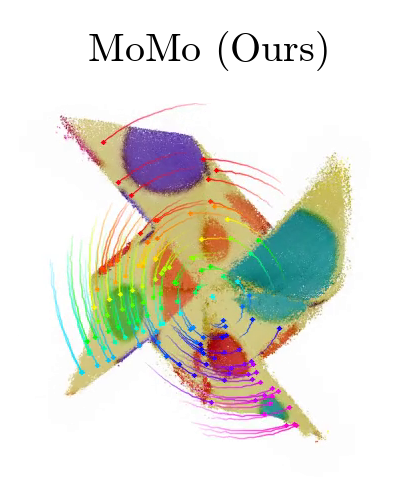
\includegraphics[width=\linewidth]{img/ours-tracks}
    \caption{Ours}
  \end{subfigure}
  \hfill
  \begin{subfigure}[b]{0.49\linewidth}
    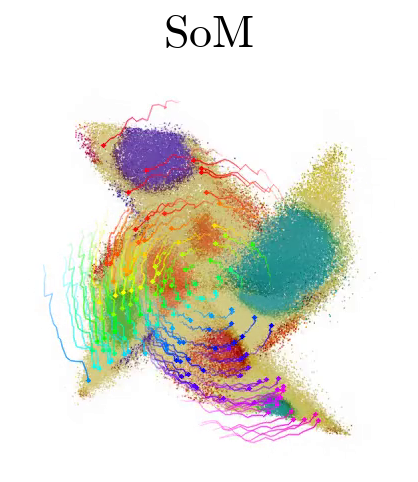
\includegraphics[width=\linewidth]{img/som-tracks}
    \caption{Shape of Motion}
  \end{subfigure}
  \caption{\lulu{Update with new MoMo} Comparison of estimated 3D tracks.}
  \label{fig:synthetic-tracks}
\end{figure}

For the synthetic pinwheel scene, we show tracks obtained from SoM~\cite{wang2025shape} and our method.
SoM-produced tracks display jitters across the tracks, while our method faithfully recovers the main rotational motion.

% fig/qualitative_comparison.tex is input at the top of sec/4_method.tex (two-column float; from here it would land after the references)
%We report quantitative and qualitative results on the DyCheck~\cite{gao2022dynamic} dataset, comparing against SoM~\cite{wang2025shape} as our main baseline, using \todo{PSNR, LPIPS, and SSIM} to evaluate image quality.
% \begin{table*}[t]
  \centering
  \definecolor{rowgray}{gray}{0.9}
  \setlength{\tabcolsep}{4.5pt}
  \renewcommand{\arraystretch}{1.25}
  \begin{tabular}{@{}lcccccc@{}}
    \toprule
    \textbf{Scene}
      & \shortstack{\textbf{PSNR\,$\uparrow$}\\ \textbf{SoM}} & \shortstack{\textbf{PSNR\,$\uparrow$}\\ \textbf{Ours}}
      & \shortstack{\textbf{SSIM\,$\uparrow$}\\ \textbf{SoM}} & \shortstack{\textbf{SSIM\,$\uparrow$}\\ \textbf{Ours}}
      & \shortstack{\textbf{LPIPS\,$\downarrow$}\\ \textbf{SoM}} & \shortstack{\textbf{LPIPS\,$\downarrow$}\\ \textbf{Ours}} \\
    \midrule
    \rowcolor{rowgray}
    apple          & \textbf{11.99} & 11.19          & 0.9890 & \textbf{0.9894} & 0.2299          & \textbf{0.2298} \\
    paper-windmill & 11.72          & \textbf{12.15} & 0.9723 & \textbf{0.9733} & 0.4471          & \textbf{0.4173} \\
    \rowcolor{rowgray}
    teddy          & \textbf{12.56} & 12.33          & 0.7281 & \textbf{0.7297} & \textbf{0.4630} & 0.4842          \\
    \textbf{Average} & \textbf{12.09} & 11.89        & 0.8965 & \textbf{0.8975} & 0.3800          & \textbf{0.3771} \\
    \bottomrule
  \end{tabular}
  \caption{Quantitative comparison against Shape-of-Motion (SoM)~\cite{wang2025shape} on the Apple, Paper Windmill, and Teddy scenes from the DyCheck dataset. Best result per metric is shown in \textbf{bold}.}
  \label{tab:quantitative}
\end{table*}

% \begin{table*}[t]
  \centering
  \definecolor{rowgray}{gray}{0.9}
  \setlength{\tabcolsep}{4.5pt}
  \renewcommand{\arraystretch}{1.25}
  \begin{tabular}{@{}lcccccc@{}}
    \toprule
    \textbf{Scene}
      & \shortstack{\textbf{PSNR\,$\uparrow$}\\ \textbf{SoM}} & \shortstack{\textbf{PSNR\,$\uparrow$}\\ \textbf{Ours}}
      & \shortstack{\textbf{SSIM\,$\uparrow$}\\ \textbf{SoM}} & \shortstack{\textbf{SSIM\,$\uparrow$}\\ \textbf{Ours}}
      & \shortstack{\textbf{LPIPS\,$\downarrow$}\\ \textbf{SoM}} & \shortstack{\textbf{LPIPS\,$\downarrow$}\\ \textbf{Ours}} \\
    \midrule
    \rowcolor{rowgray}
    apple          & 11.99 & \todo{\textbf{12.01}}          & 0.9890 & \textbf{0.9902} & 0.2299          & \textbf{0.2214} \\
    paper-windmill & 11.72          & \todo{\textbf{12.08}} & 0.9723 & \textbf{0.9727} & 0.4471          & \textbf{0.4195} \\
    \rowcolor{rowgray}
    \todo{teddy}          & \textbf{12.56} & 12.33          & 0.7281 & \textbf{0.7297} & \textbf{0.4630} & 0.4842          \\
    \todo{\textbf{Average}} & \textbf{12.09} & 11.89        & 0.8965 & \textbf{0.8975} & 0.3800          & \textbf{0.3771} \\
    \bottomrule
  \end{tabular}
  \caption{\todo{TMP - newer results after changes} Quantitative comparison against Shape-of-Motion (SoM)~\cite{wang2025shape} on the Apple, Paper Windmill, and Teddy scenes from the DyCheck dataset. Best result per metric is shown in \textbf{bold}.}
  \label{tab:quantitative}
\end{table*}


We also provide qualitative results on the DyCheck~\cite{gao2022dynamic} benchmark (Fig.~\ref{fig:qualitative-comparison}. 
At the same number of bases ($B=20$), our method achieves higher reconstruction quality than SoM, with strong regularization still holding at this basis count, while SoM shows clear overfitting and degraded test-view quality. In the `Paper Windmill' scene specifically, a real video version of our synthetic example, the recovered Gaussian tracks show our method preserving the dominant windmill-rotation motion, while SoM produces per-Gaussian overfitted tracks that fail to capture this coherent motion.

% fig/tab_full_dycheck.tex and fig/tab_full_nvidia.tex are input in the supplementary, sec/X_suppl.tex ([Claude] 2026-11-05, user request)
% [Claude] 2026-11-05: motion-coefficient comparison moved up from the end of the section, before the line plots (user request).
% [Claude] 2026-10-28: placeholder for the motion-coefficient comparison (user request); grey boxes stand in for the images.
% [Claude] 2026-11-05 (user requests): apple (seed 44), Balloon1 (seed 43) and teddy (seed 43) at the first training frame (0_00000), spin (seed 42)
% at training frame 0_00270 (18 s into the 15 fps render). Coefficients = that frame of tests/render_coefs.py's renders (outputs/bdf/modes_vis/
% {som/<S>/bases_10,split_init/<S>/bases_<B>}[_s<seed>]/videos/epoch_0499/motion_coefs.mp4, right half); input = the dataset's training image,
% cropped like the render (Balloon1: 458 x 240 of 470 x 248; DyCheck 720 x 960, uncropped).
\begin{figure}[t]
  \centering
  \newcommand{\coefrow}[3]{\rotatebox{90}{\makebox[#2\linewidth][c]{\footnotesize #3}} & \coefimg{coef_#1_input} & \coefimg{coef_#1_som10} &
    \coefimg{coef_#1_ours} \\}
  \newcommand{\coefimg}[1]{\includegraphics[width=0.3\linewidth]{img/#1}}
  \setlength{\tabcolsep}{1pt}
  \begin{tabular}{@{}c@{\hspace{2pt}}ccc@{}}
    \coefrow{apple_s44_f0}{0.4}{Apple}
    \coefrow{Balloon1_s43_f0}{0.157}{Balloon1}
    \coefrow{teddy_s43_f0}{0.4}{Teddy}
    \coefrow{spin_s42_f270}{0.4}{Spin}
     & \makebox[0.3\linewidth][c]{\footnotesize Input} &
       \makebox[0.3\linewidth][c]{\footnotesize SoM-10} &
       \makebox[0.3\linewidth][c]{\footnotesize Ours} \\
  \end{tabular}
  \caption{\claudetag\ Motion coefficients of Shape of Motion~\cite{wang2025shape} with its default 10 bases and of our method
    ($B$ from its stopping rule: 5 on apple, 4 on Balloon1, 8 on teddy, 9 on spin), rendered from a training view: the first one for
    apple (DyCheck, seed 44), Balloon1 (NVIDIA, seed 43) and teddy (DyCheck, seed 43), frame 270 for spin (DyCheck, seed 42). Each
    foreground Gaussian is coloured by its blending weights: every basis of a model has its own hue, spaced evenly over that model's
    bases, and mixed weights mix the hues; the background is grey. Hues are not matched between the two methods: what matters is which
    parts share one colour.}
  \label{fig:coef-comparison}
\end{figure}

\Cref{fig:coef-comparison} compares the motion coefficients of Shape of Motion and our method.
\todo{discuss once the images exist.}

% Claude, generated by tests/plot_som_sweep_iphone.py --average --scenes apple teddy spin paper-windmill block --name iphone_avg
% (branch bd-split-rules): SoM rerun on the current code (seed 42, B = 1..10) averaged over the five iPhone scenes at each B; ours
% (seed 42) at the mean of its per-scene B (apple 5, teddy 8, spin 9, paper-windmill 9, block 7); open circle = SoM averaged at
% each scene's B.
% [Claude] 2026-11-05 (user request): validation only, one panel per dataset, Fig. 2b style, MoMo final (split_init at the tables' B:
% DyCheck 5 8 9 9 10, NVIDIA 4 6 8 7 5 6 6). tests/plot_sweep_val_avg.py -> plots/sweep_val_avg/sweep_val_{dycheck,nvidia}.pdf (copied to img/).
% Seed 42, last epoch, val/fg_psnr. DyCheck SoM sweep: outputs/bdf/som; NVIDIA SoM sweep: the Killarney sweep (outputs/bdf_nvsweep, parity
% with Vulcan within 0.1 dB). Values: DyCheck MoMo 12.64 at B 8.2, SoM at each B 12.64, SoM-10 12.63, SoM peak 12.74 at B 3;
% NVIDIA MoMo 20.42 at B 6.0, SoM at each B 20.19, SoM-10 20.32, SoM max 20.38 at B 9.
\begin{figure}[t]
  \centering
  \begin{subfigure}{\linewidth}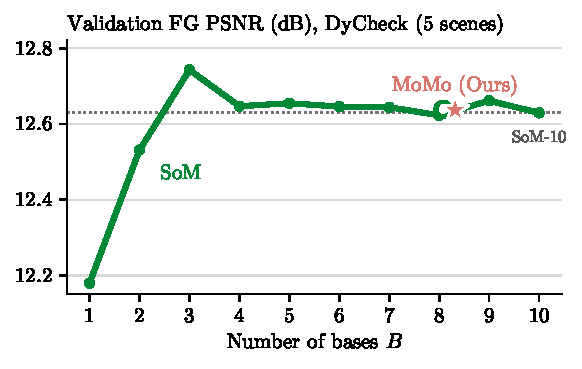
\includegraphics[width=\linewidth]{img/sweep_val_dycheck.pdf}\phantomsubcaption\label{fig:sweep-avg-dycheck}\end{subfigure}\\[2pt]
  \begin{subfigure}{\linewidth}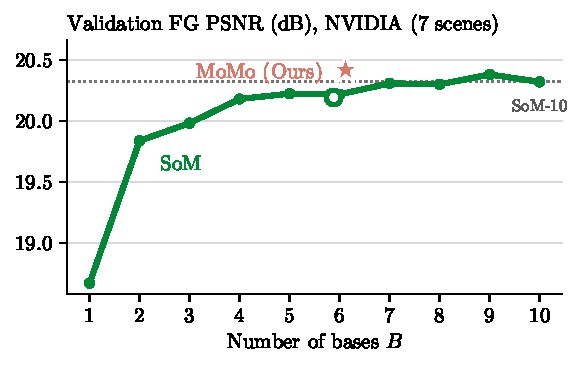
\includegraphics[width=\linewidth]{img/sweep_val_nvidia.pdf}\phantomsubcaption\label{fig:sweep-avg-nvidia}\end{subfigure}
  \caption{\claudetag\ Foreground PSNR on the held-out views against the number of bases, averaged over the five DyCheck
    (iPhone) scenes (top) and the seven NVIDIA scenes (bottom): SoM~\cite{wang2025shape} with $B = 1$--$10$ bases (curve), ours at
    the mean of the $B$ its stopping rule picks per scene (star; 8.2 on DyCheck, 6.0 on NVIDIA) and SoM given each scene's $B$
    (circle); dotted line: SoM-10. Seed 42.}
  \label{fig:sweep-avg}
\end{figure}

% % Claude, generated by tests/plot_track_error_vs_bases.py --average (branch bd-split-rules): track error (masked L1, SoM's track
% loss) of the initialisation, before photometric training, seed 42, mean over apple, teddy, spin, paper-windmill and block.
% SoM init (k-means + Procrustes + 1000 Adam iterations) at B = 1..10; MoMo with its own 5 % rule (B = 6, 9, 9, 6, 7).
\begin{figure}[t]
  \centering
  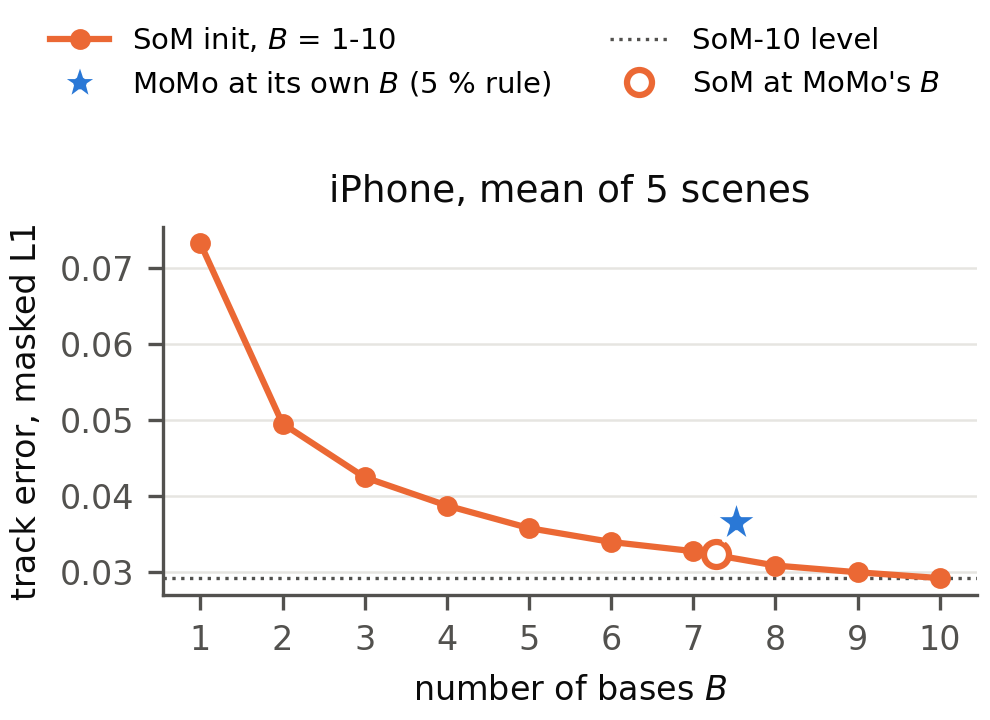
\includegraphics[width=\linewidth]{img/track_error_iphone_avg.png}
  \caption{\claudetag\ \claudeadd{Track error of the initialization (masked $\ell_1$ distance to the 3D tracks, before photometric
    training) against the number of bases, averaged over the five DyCheck (iPhone) scenes: SoM~\cite{wang2025shape} with
    $B = 1$--$10$ bases (curve), MoMo with the number of bases its $\tau = 0.05$ cutoff chooses (star) and SoM with that same number
    (circle); dotted line: SoM-10. Lower is better. Seed 42.}}
  \label{fig:track-avg}
\end{figure}
   % [Claude] 2026-11-05: Fig. 6 (track error vs. number of bases) removed (user request); the file is kept
% [Claude] 2026-11-04: inside the pending \claudedel below, \todo{...} became \textcolor{red}{TODO:} + plain text, because \sout cannot break a braced argument and the line ran 107pt into the margin; same words.
\Cref{tab:full-dycheck,tab:full-nvidia} compare our method (\cref{sec:split-init}) on the full held-out views with SoM~\cite{wang2025shape}
at its default 10 bases (SoM-10) and with as many bases as ours (SoM-$B$). On DyCheck, with
8.2 bases on average, ours is level with both in PSNR ($-0.01$\,dB against SoM-$B$, $-0.03$\,dB against SoM-10) and ahead in
LPIPS ($-0.003$ and $-0.002$) and SSIM. On NVIDIA, with 6.0 bases on average, ours is again level, $+0.01$\,dB against SoM-$B$ and
$-0.02$\,dB against SoM-10 with an LPIPS 0.002 higher: it is ahead on Truck ($+0.20$\,dB against SoM-10) and Umbrella ($+0.02$\,dB) and
behind SoM-10 by 0.03--0.12\,dB on the other five scenes. The residual-pattern clustering is what makes the coefficients separate the
moving parts (one basis per person in Jumping, the toy's legs in teddy); without it (movers = the whole poorly fitted half,
$\ell_1$ residual) the coefficients blend neighbouring parts, at $+0.07$\,dB PSNR on DyCheck and $+0.02$\,dB on NVIDIA
(paired over 13 and 20 runs).
\Cref{fig:sweep-avg} averages the trade-off over the scenes of each
dataset, on the held-out views (foreground PSNR, seed 42). On DyCheck, SoM peaks at 12.74\,dB at three bases and stays near 12.65\,dB
from then on (12.63\,dB at ten); ours, at 8.2 bases on average, scores 12.64\,dB, level with SoM given each scene's number of bases
(12.64\,dB) and with SoM-10. On NVIDIA, SoM rises to 20.2--20.4\,dB from four bases on (20.32\,dB at ten); ours, at 6.0 bases on
average, scores 20.42\,dB, above SoM given each scene's number of bases (20.19\,dB) and SoM-10.
% [Claude] 2026-11-05 (user request): Fig. 2b on the real scenes. tests/plot_scene_avg_coef.py -> plots/scene_avg_coef/avg_blending_weight_
% {nvidia,dycheck}_sorted.pdf (copied to img/): average softmax blending weight per basis, ours (split_init at the tables' B) vs SoM-10, mean over
% seeds 42-44 (block SoM: 42 / 43), each run's bases sorted by weight; rank k averaged over the scenes that have it (ours: NVIDIA 7 7 7 7 6 5 2 1,
% DyCheck 5 5 5 5 5 4 4 4 3 1). Curves: NVIDIA ours 0.372 0.244 0.174 0.104 0.070 0.043 0.037 0.034, SoM-10 0.190 0.158 0.133 0.112 0.097 0.087
% 0.074 0.058 0.050 0.042; DyCheck ours 0.375 0.183 0.123 0.087 0.072 0.069 0.054 0.042 0.037 0.038, SoM-10 0.182 0.146 0.122 0.111 0.102 0.087
% 0.075 0.068 0.060 0.046 (top values to 4 decimals: 0.3719 / 0.1897 NVIDIA, 0.3746 / 0.1824 DyCheck).
% [Claude] 2026-11-05: NVIDIA panel switched from native to sorted order (user request), restored after a concurrent edit reverted it.
\begin{figure}[t]
  \centering
  \begin{subfigure}{\linewidth}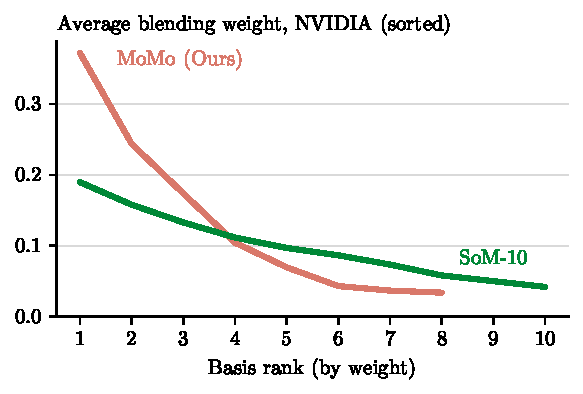
\includegraphics[width=\linewidth]{img/avg_blending_weight_nvidia_sorted.pdf}\phantomsubcaption\label{fig:avg-weight-nvidia}\end{subfigure}\\[2pt]
  \begin{subfigure}{\linewidth}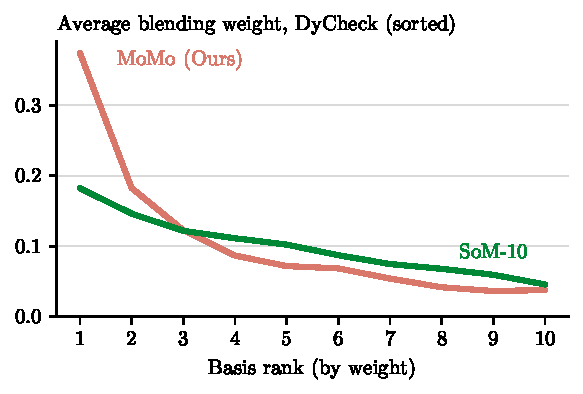
\includegraphics[width=\linewidth]{img/avg_blending_weight_dycheck_sorted.pdf}\phantomsubcaption\label{fig:avg-weight-dycheck}\end{subfigure}
  \caption{Average blending weight of each basis on the real scenes: ours with the
    $B$ its stopping rule picks per scene against SoM~\cite{wang2025shape} with its default 10 bases (SoM-10), mean over three seeds and
    over the scenes, with each model's bases sorted by weight, which does not depend on SoM's arbitrary basis order. Top: the seven
    NVIDIA scenes. Bottom: the five DyCheck scenes. A rank is averaged over the scenes that have it, so ours ends at the largest $B$ of
    the dataset.}
  \label{fig:avg-weight-real}
\end{figure}

\Cref{fig:avg-weight-real} shows the average blending weight of each basis on the real scenes. Ours concentrates the weight on
few bases: with the bases sorted by weight, its strongest basis carries 0.37 of the weight on both datasets, against 0.19 (NVIDIA) and
0.18 (DyCheck) for SoM-10, and its three strongest carry 0.79 and 0.68 against 0.48 and 0.45.
We compare the two initializations on the 3D tracks alone, % [Claude] 2026-11-05: the struck reference was \Cref, written as Fig.~\ref because \sout cannot process \cref
 with MoMo choosing its number of bases by the
$\tau = 0.05$ cutoff (6, 9, 9, 6 and 7 bases on apple, teddy, spin, paper-windmill and block; 7.4 on average). MoMo's initialization does
not fit the tracks more tightly than SoM's: at the same number of bases its masked $\ell_1$ track error is 13\,\% higher on
average and higher on every scene. Trained with these $B$ (seed 42), MoMo reaches 16.75\,dB PSNR on the held-out views on average, 0.08\,dB below SoM
given the same $B$ and 0.06\,dB below SoM-10, with a slightly lower LPIPS (0.386 against 0.388 and 0.390); the gap is
within the seed spread and comes mostly from spin. On NVIDIA the $\tau$ cutoff chooses 5.6 bases on average (5, 4, 9, 6, 5, 4 and 6 on
Balloon1, Balloon2, Jumping, Playground, Skating, Truck and Umbrella); the initialization's track error is again higher than
SoM's at the same $B$ (by 14\,\% on average and on every scene), yet after training MoMo is 0.11\,dB above SoM given the same
$B$ (23.37 against 23.26\,dB) and 0.03\,dB below SoM-10 (23.40\,dB), with LPIPS 0.101 against 0.102 and 0.100.
\Cref{tab:full-dycheck,tab:full-nvidia} use, for each scene, the $B$ the $\tau = 0.05$ cutoff picks with the current initialization (seed 42).

% [Claude] 2026-10-28: comparison with prior work, placeholder (user request); table in fig/tab_sota_nvs.tex.
% [Claude] 2026-10-28: placeholder comparison with prior work on novel view synthesis, laid out like MotionScale's table (user
% screenshot), ours as the last row. Only our own runs (user 2026-10-28): Shape of Motion = our SoM-10 reruns and ours = the candidate
% default, both the average rows of fig/tab_full_{dycheck,nvidia}.tex (DyCheck: 4 of 5 scenes, block pending). MoSca trained but was not
% scored, Gaussian Marbles / HiMoR training crashed (missing LPIPS alex.pth), MotionScale not run: TODO.
% [Claude] 2026-11-05: Ours re-synced with those average rows, which are MoMo (L2 + clustering + 5 % cutoff, user 2026-11-04) since
% 2026-11-04; this row still held the old MoMo (energy + L1). NVIDIA now includes Umbrella at the rule's B = 6 (Killarney runs).
% [Claude] 2026-11-04: NVIDIA baselines trained on Killarney (seed 42), scored on Vulcan by one evaluator,
% scripts/iphone_data_diag/eval_nv.py (SoM's mPSNR / mSSIM / mLPIPS, i.e. our validator's metric code, mask = covisible/2x/val):
% MoSca (tto_test renders; its own test_covisible masks are byte-identical copies of ours), MotionScale, HiMoR (its own scorer masks by
% render alpha: 23.31 / 0.749 / 0.105, not used). GM: its exported renders are blank (render half of every image is black), so its own
% in-pipeline FINAL_VAL masked metrics are used: same covisible/2x/val mask, DyCheck metric definitions (unmasked 22.56 / 0.711 / 0.128
% not used). Per-scene numbers: tmp/mosca_check/nveval_2131545.out (main checkout); CHANGELOG 2026-11-04.
% [Claude] 2026-11-05: MoSca re-rendered at the GT val poses WITHOUT its test-time pose optimisation (TTO), like every other method
% (tmp/mosca_check/mosca_eval_notto.py, job 2137456): 22.80 / 0.716 / 0.118. Its TTO chains each frame's pose from the previous frame's
% optimised one, so on our static val cameras the poses wandered by up to 4.6 deg (tto_drift.py) -> the old 21.59 / 0.646 / 0.147.
% [Claude] 2026-11-05: DyCheck scored at full resolution, 720x960 (user decision), by eval_nv.py with flow3d_preprocessed/covisible/1x/val
% (job 2137519, tmp/mosca_check/dycheckeval_2137519.out; SoM-10 seed 42 there = 16.81, as in the table). HiMoR (fixed cameras): 16.04 /
% 0.554 / 0.445. MoSca refines its iPhone train cameras (0.3-0.6 deg median, cam_drift_iphone.py), so it is rendered with that per-frame
% correction carried to the val camera (as MotionScale's validator does; ours and HiMoR keep their cameras fixed, correction = 0):
% 17.16 / 0.569 / 0.502 (job 2137974, mosca_eval_corr.py; raw given cameras 15.60, its test-time pose optimisation 18.61: not used).
% NVIDIA check: the corrected renders match the no-TTO ones (Skating 27.53 vs 27.54). MotionScale: block / teddy resuming; GM: reruns
% with the LPIPS fix pending.
\begin{table}[t]
  \centering
  \resizebox{\linewidth}{!}{%
  \begin{tabular}{@{}lcccccc@{}}
    \toprule
     & \multicolumn{3}{c}{DyCheck NVS} & \multicolumn{3}{c}{NVIDIA NVS} \\
    \cmidrule(lr){2-4} \cmidrule(l){5-7}
    Method & PSNR\,$\uparrow$ & SSIM\,$\uparrow$ & LPIPS\,$\downarrow$ & PSNR\,$\uparrow$ & SSIM\,$\uparrow$ & LPIPS\,$\downarrow$ \\
    \midrule
    Shape of Motion~\cite{wang2025shape} & 16.81 & 0.638 & 0.389 & 23.40 & 0.749 & 0.100 \\
    MoSca~\cite{lei2025mosca} & 17.16 & 0.569 & 0.502 & 22.80 & 0.716 & 0.118 \\
    Gaussian Marbles~\cite{stearns2024dynamic} & \textcolor{red}{TODO} & \textcolor{red}{TODO} & \textcolor{red}{TODO} & 23.61 & 0.778 & 0.087 \\
    MotionScale~\cite{zhou2026motionscale} & \textcolor{red}{TODO} & \textcolor{red}{TODO} & \textcolor{red}{TODO} & 22.20 & 0.678 & 0.155 \\
    HiMoR~\cite{liang2025himor} & 16.04 & 0.554 & 0.445 & 23.35 & 0.748 & 0.101 \\
    \midrule
    Ours & 16.79 & 0.639 & 0.387 & 23.38 & 0.748 & 0.102 \\
    \bottomrule
  \end{tabular}}
  \caption{\ Novel view synthesis on the held-out views of DyCheck (iPhone)~\cite{gao2022dynamic} and NVIDIA Dynamic
    Scenes~\cite{yoon2020novel}. \textcolor{red}{TODO: missing methods.} All scores are computed on the covisible pixels with the dataset's covisibility masks and the same metric code (masked
    PSNR, SSIM and LPIPS as in DyCheck)}
  \label{tab:sota-nvs}
\end{table}

\Cref{tab:sota-nvs} compares our method with prior monocular dynamic reconstruction methods on novel view synthesis.
\todo{discuss once the missing entries are in.}

% [Claude] 2026-10-28: memory / speed placeholder (user request); table in fig/tab_efficiency.tex.
% [Claude] 2026-10-28: placeholder for the memory / speed comparison (user request); same methods and order as fig/tab_sota_nvs.tex,
% ours as the last row. Every cell TODO.
\begin{table}[t]
  \centering
  \resizebox{\linewidth}{!}{%
  \begin{tabular}{@{}lccccc@{}}
    \toprule
    Method & Formula & \#Params\,$\downarrow$ & Memory (disk)\,$\downarrow$ & RAM\,$\downarrow$ & NVS inference time\,$\downarrow$ \\
    \midrule
    Shape of Motion~\cite{wang2025shape} & $24G + 90T$ & 1.81M & \textcolor{red}{TODO} & \textcolor{red}{TODO} & \textcolor{red}{TODO} \\
    MoSca~\cite{lei2025mosca} & \textcolor{red}{TODO} & \textcolor{red}{TODO} & \textcolor{red}{TODO} & \textcolor{red}{TODO} & \textcolor{red}{TODO} \\
    Gaussian Marbles~\cite{stearns2024dynamic} & \textcolor{red}{TODO} & \textcolor{red}{TODO} & \textcolor{red}{TODO} & \textcolor{red}{TODO} & \textcolor{red}{TODO} \\
    MotionScale~\cite{zhou2026motionscale} & \textcolor{red}{TODO} & \textcolor{red}{TODO} & \textcolor{red}{TODO} & \textcolor{red}{TODO} & \textcolor{red}{TODO} \\
    HiMoR~\cite{liang2025himor} & \textcolor{red}{TODO} & \textcolor{red}{TODO} & \textcolor{red}{TODO} & \textcolor{red}{TODO} & \textcolor{red}{TODO} \\
    \midrule
    Ours & $(14 + B)\,G + 9BT$ & 1.36M & \textcolor{red}{TODO} & \textcolor{red}{TODO} & \textcolor{red}{TODO} \\
    \bottomrule
  \end{tabular}}
  \caption{\claudetag\ Memory and speed of each method: the parameter count of the dynamic foreground as a formula and its value,
    the size of the trained model on disk, RAM, and the time to render a novel view. $G$: foreground Gaussians (14 parameters each, plus one
    blending weight per basis); $B$: bases (9 parameters per frame each); $T$: frames. Shape of Motion uses $B = 10$; ours chooses $B$ per
    scene. Values: average over the DyCheck (iPhone) scenes. \textcolor{red}{TODO: remaining entries; units and measurement setup.}}
  \label{tab:efficiency}
\end{table}

Our method finds the optimally efficient number of motion bases tailored to each scene, leading to a reduction in the number of parameters. In addition to the standard Gaussian parameters (3 for the center, 4 for the rotation quaternion, 3 for the scale, 1 for the opacity and 3 for the color, 14 in total), each Gaussian stores $B$ time-invariant basis coefficients. Each motion basis stores 6 rotation and 3 translation parameters per frame. Thus, in total, MoMo requires $G \times (14 + B) + B \times T \times 9$ parameters to represent a scene, where $G$ is the number of foreground Gaussians only, and $G \gg T \gg B$. Naively training a static 3DGS scene per frame would require $G \times T \times 14$ parameters. Our method reduces the number of parameters compared to SoM~\cite{wang2025shape} by reducing $B$. On the dynamic part of the scene, our method on average stores 1.36M parameters on the iPhone dataset while SoM-10 stores 1.81M, which is a 25\% reduction in the number of parameters. \Cref{tab:efficiency} presents the memory cost and parameter count of other methods. \lulu{25\% is from us having fewer Gaussians too, purely from formula should be 11\%}% [Claude] 2026-11-05: escaped the two % signs; an unescaped % comments out the rest of the line, closing brace included



% [Claude] 2026-10-28: cutoff sweep placeholder (user request); the table is in fig/tab_eps_sweep.tex.
% [Claude] 2026-10-28: placeholder for the sweep of the cutoff epsilon of the stopping rule (user request). Candidate default
% (split_init_only45e_l1). [Claude] 2026-10-29: every row = MoMo with the rule at that epsilon, seed 42, last epoch
% (metrics_imgs.json of outputs/bdf/split_init_only45e_l1_gNN/<scene>/bases_20, NN = 100 x epsilon), mean over the scenes; B = mean
% chosen_N.txt. iPhone per-scene B: 0.05 6 9 9 6 7 | 0.10 4 5 6 5 5 | 0.20 3 4 4 4 4 (apple teddy spin paper-windmill block).
% NVIDIA (trained on Killarney, results in outputs/bdf_nvsweep; parity with Vulcan within 0.1 dB) per-scene B, Balloon1 Balloon2
% Jumping Playground Skating Truck Umbrella-fixed: 0.01 8 11 18 13 9 16 20 | 0.02 6 7 12 8 7 11 10 | 0.05 5 4 9 6 5 4 6 |
% 0.10 3 4 5 5 4 3 4 | 0.20 2 3 4 4 3 3 3. iPhone 0.01: 19 20 15 11 20 | 0.02: 11 13 12 9 14.
% [Claude] 2026-10-29 evening: rows 0.001 / 0.005 / 0.50 / 0.75 added (user request; folders g001 / g005 / g50 / g75 = the digits
% after "0."). iPhone trained on Vulcan (bd-split-rules CHANGELOG); NVIDIA = Killarney step 2c, still TODO. [Claude] 2026-10-30: iPhone
% filled; per-scene B (apple teddy spin paper-windmill block) 0.001: 20 20 20 20 20 | 0.005: 20 20 20 14 20 | 0.50: 2 2 2 2 2 | 0.75: 2 2 2 2 2.
\begin{table}[t]
  \centering
  \footnotesize
  % [Claude] 2026-10-28: B, SSIM and LPIPS columns added (user request); \resizebox so that the nine columns fit one column.
  \resizebox{\linewidth}{!}{%
  \begin{tabular}{@{}lcccccccc@{}}
    \toprule
     & \multicolumn{2}{c}{$B$} & \multicolumn{2}{c}{PSNR\,$\uparrow$} & \multicolumn{2}{c}{SSIM\,$\uparrow$} & \multicolumn{2}{c}{LPIPS\,$\downarrow$} \\
    \cmidrule(lr){2-3} \cmidrule(lr){4-5} \cmidrule(lr){6-7} \cmidrule(l){8-9}
    $\tau$ & NVIDIA & iPhone & NVIDIA & iPhone & NVIDIA & iPhone & NVIDIA & iPhone \\
    \midrule
    0.001 & \textcolor{red}{TODO} & 20.0 & \textcolor{red}{TODO} & 16.80 & \textcolor{red}{TODO} & 0.638 & \textcolor{red}{TODO} & 0.384 \\
    0.005 & \textcolor{red}{TODO} & 18.8 & \textcolor{red}{TODO} & 16.76 & \textcolor{red}{TODO} & 0.638 & \textcolor{red}{TODO} & 0.385 \\
    0.01 & 13.6 & 17.0 & 23.44 & 16.78 & 0.750 & 0.637 & 0.098 & 0.384 \\
    0.02 & 8.7 & 11.8 & 23.39 & 16.72 & 0.748 & 0.637 & 0.100 & 0.386 \\
    0.05 & 5.6 & 7.4 & 23.37 & 16.75 & 0.747 & 0.638 & 0.101 & 0.386 \\
    0.10 & 4.0 & 5.0 & 23.37 & 16.86 & 0.747 & 0.639 & 0.102 & 0.387 \\
    0.20 & 3.1 & 3.8 & 23.32 & 16.84 & 0.745 & 0.639 & 0.104 & 0.385 \\
    0.50 & \textcolor{red}{TODO} & 2.0 & \textcolor{red}{TODO} & 16.69 & \textcolor{red}{TODO} & 0.638 & \textcolor{red}{TODO} & 0.398 \\
    0.75 & \textcolor{red}{TODO} & 2.0 & \textcolor{red}{TODO} & 16.67 & \textcolor{red}{TODO} & 0.637 & \textcolor{red}{TODO} & 0.397 \\
    \bottomrule
  \end{tabular}}
  \caption{\claudetag\ Validation PSNR, SSIM and LPIPS of our method and its number of bases $B$ on the held-out views of NVIDIA
    Dynamic Scenes~\cite{yoon2020novel} and DyCheck (iPhone)~\cite{gao2022dynamic} for several values of the $\tau$ cutoff
    (\cref{sec:tau}). Covisible pixels, seed 42; every entry, $B$ included, is averaged over the scenes
    (iPhone: all five, block included). At every $\tau$ our method chooses $B$ itself with the cutoff. $\tau = 0.05$ is the value used in all
    other experiments.}
  \label{tab:eps-sweep}
\end{table}

\Cref{tab:eps-sweep} varies the $\tau$ cutoff (\cref{sec:tau}): the basis growth ends once an added basis lowers the weighted 3D track error by less than a fraction $\tau$.
On DyCheck a looser cutoff stops earlier and renders slightly better: $\tau = 0.10$ ($B = 5.0$) and $0.20$ ($B = 3.8$) are 0.11 and 0.09\,dB above $\tau = 0.05$ ($B = 7.4$), mostly from spin and apple, while block loses 0.14--0.20\,dB; SSIM and LPIPS change by at most 0.002. Tighter cutoffs do not help either: $\tau = 0.02$ ($B = 11.8$) and $0.01$ ($B = 17.0$) score 16.72 and 16.78\,dB, so on DyCheck PSNR is not monotone in $B$.
On NVIDIA the trend reverses but stays as small: a tighter cutoff grows more bases and scores slightly higher, from 23.32\,dB at $\tau = 0.20$ ($B = 3.1$) to 23.44\,dB at $\tau = 0.01$ ($B = 13.6$), with $\tau = 0.05$ at 23.37\,dB ($B = 5.6$). Across the cutoffs the held-out PSNR moves by at most 0.14\,dB on either dataset while the mean $B$ changes more than fourfold, so the method is not sensitive to $\tau$; $\tau = 0.05$ sits between the two datasets' preferences.
\claudenote{Every row of \cref{tab:eps-sweep}, 0.05 included, lets the $\tau$ cutoff choose $B$ (seed 42). According to the table's source comment, these runs (\texttt{split\_init\_only45e\_l1\_gNN}) use the previous initialization (no residual-pattern clustering, $\ell_1$ residual), while \cref{tab:full-dycheck,tab:full-nvidia} use the current one over three seeds, so the 0.05 row is not their average row and the sweep would need rerunning with the current initialization.}

% [Claude] 2026-11-05: moved up, before % Claude, generated by tests/plot_som_sweep_iphone.py --average --scenes apple teddy spin paper-windmill block --name iphone_avg
% (branch bd-split-rules): SoM rerun on the current code (seed 42, B = 1..10) averaged over the five iPhone scenes at each B; ours
% (seed 42) at the mean of its per-scene B (apple 5, teddy 8, spin 9, paper-windmill 9, block 7); open circle = SoM averaged at
% each scene's B.
% [Claude] 2026-11-05 (user request): validation only, one panel per dataset, Fig. 2b style, MoMo final (split_init at the tables' B:
% DyCheck 5 8 9 9 10, NVIDIA 4 6 8 7 5 6 6). tests/plot_sweep_val_avg.py -> plots/sweep_val_avg/sweep_val_{dycheck,nvidia}.pdf (copied to img/).
% Seed 42, last epoch, val/fg_psnr. DyCheck SoM sweep: outputs/bdf/som; NVIDIA SoM sweep: the Killarney sweep (outputs/bdf_nvsweep, parity
% with Vulcan within 0.1 dB). Values: DyCheck MoMo 12.64 at B 8.2, SoM at each B 12.64, SoM-10 12.63, SoM peak 12.74 at B 3;
% NVIDIA MoMo 20.42 at B 6.0, SoM at each B 20.19, SoM-10 20.32, SoM max 20.38 at B 9.
\begin{figure}[t]
  \centering
  \begin{subfigure}{\linewidth}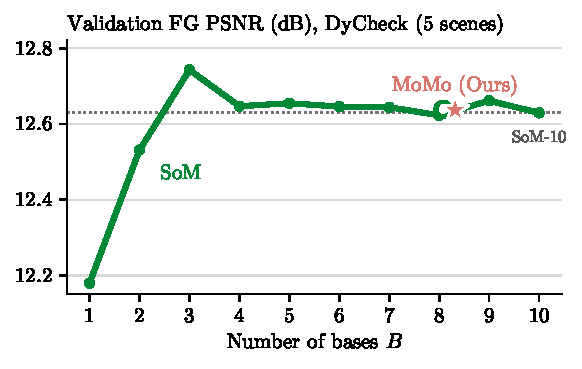
\includegraphics[width=\linewidth]{img/sweep_val_dycheck.pdf}\phantomsubcaption\label{fig:sweep-avg-dycheck}\end{subfigure}\\[2pt]
  \begin{subfigure}{\linewidth}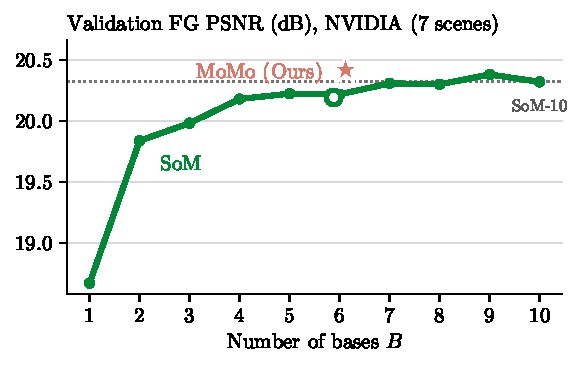
\includegraphics[width=\linewidth]{img/sweep_val_nvidia.pdf}\phantomsubcaption\label{fig:sweep-avg-nvidia}\end{subfigure}
  \caption{\claudetag\ Foreground PSNR on the held-out views against the number of bases, averaged over the five DyCheck
    (iPhone) scenes (top) and the seven NVIDIA scenes (bottom): SoM~\cite{wang2025shape} with $B = 1$--$10$ bases (curve), ours at
    the mean of the $B$ its stopping rule picks per scene (star; 8.2 on DyCheck, 6.0 on NVIDIA) and SoM given each scene's $B$
    (circle); dotted line: SoM-10. Seed 42.}
  \label{fig:sweep-avg}
\end{figure}
 (user request); the old copy's \input is commented out and its text
% struck, with \Cref written as Fig.~\ref because \sout cannot process \cref.
% % [Claude] 2026-10-28: placeholder for the motion-coefficient comparison (user request); grey boxes stand in for the images.
% [Claude] 2026-11-05 (user requests): apple (seed 44), Balloon1 (seed 43) and teddy (seed 43) at the first training frame (0_00000), spin (seed 42)
% at training frame 0_00270 (18 s into the 15 fps render). Coefficients = that frame of tests/render_coefs.py's renders (outputs/bdf/modes_vis/
% {som/<S>/bases_10,split_init/<S>/bases_<B>}[_s<seed>]/videos/epoch_0499/motion_coefs.mp4, right half); input = the dataset's training image,
% cropped like the render (Balloon1: 458 x 240 of 470 x 248; DyCheck 720 x 960, uncropped).
\begin{figure}[t]
  \centering
  \newcommand{\coefrow}[3]{\rotatebox{90}{\makebox[#2\linewidth][c]{\footnotesize #3}} & \coefimg{coef_#1_input} & \coefimg{coef_#1_som10} &
    \coefimg{coef_#1_ours} \\}
  \newcommand{\coefimg}[1]{\includegraphics[width=0.3\linewidth]{img/#1}}
  \setlength{\tabcolsep}{1pt}
  \begin{tabular}{@{}c@{\hspace{2pt}}ccc@{}}
    \coefrow{apple_s44_f0}{0.4}{Apple}
    \coefrow{Balloon1_s43_f0}{0.157}{Balloon1}
    \coefrow{teddy_s43_f0}{0.4}{Teddy}
    \coefrow{spin_s42_f270}{0.4}{Spin}
     & \makebox[0.3\linewidth][c]{\footnotesize Input} &
       \makebox[0.3\linewidth][c]{\footnotesize SoM-10} &
       \makebox[0.3\linewidth][c]{\footnotesize Ours} \\
  \end{tabular}
  \caption{\claudetag\ Motion coefficients of Shape of Motion~\cite{wang2025shape} with its default 10 bases and of our method
    ($B$ from its stopping rule: 5 on apple, 4 on Balloon1, 8 on teddy, 9 on spin), rendered from a training view: the first one for
    apple (DyCheck, seed 44), Balloon1 (NVIDIA, seed 43) and teddy (DyCheck, seed 43), frame 270 for spin (DyCheck, seed 42). Each
    foreground Gaussian is coloured by its blending weights: every basis of a model has its own hue, spaced evenly over that model's
    bases, and mixed weights mix the hues; the background is grey. Hues are not matched between the two methods: what matters is which
    parts share one colour.}
  \label{fig:coef-comparison}
\end{figure}


% \begin{figure}[t]
  \centering
  \begin{subfigure}[b]{0.48\linewidth}
    \centering
    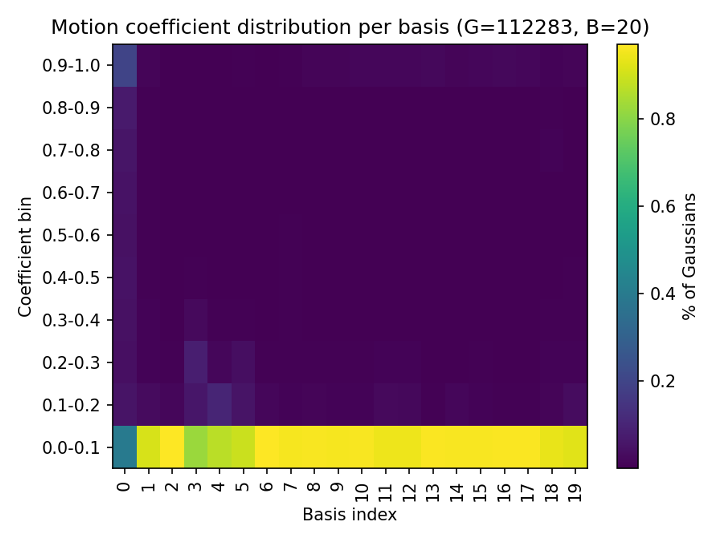
\includegraphics[width=\linewidth]{img/basis_distribution_ours.png}
    \caption{Ours}
    \label{fig:basis-distribution-ours}
  \end{subfigure}
  \hfill
  \begin{subfigure}[b]{0.48\linewidth}
    \centering
    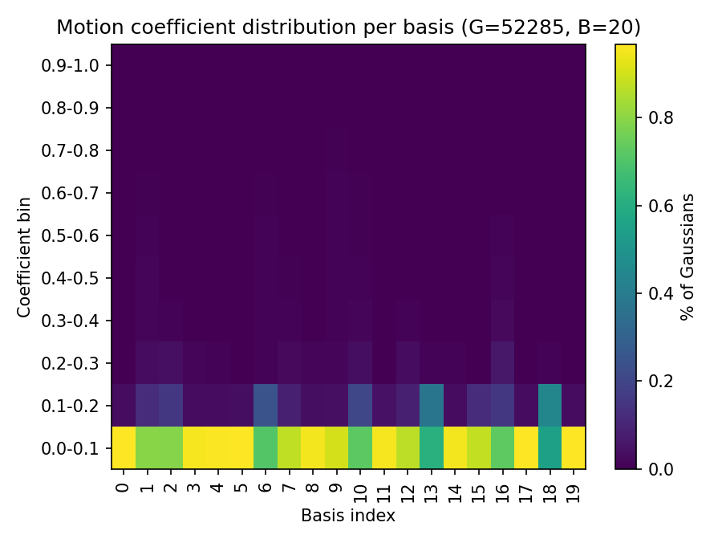
\includegraphics[width=\linewidth]{img/basis_distribution_som.png}
    \caption{Shape-of-Motion}
    \label{fig:basis-distribution-som}
  \end{subfigure}
  \caption{Distribution of motion basis coefficients after softmax. }
  \label{fig:basis-distribution}
\end{figure}

% Figure~\ref{fig:basis-distribution} shows that the motion bases coefficients trained using our method concentrate around the first basis at initialization, and the remaining bases are mostly used for local correction.
% In comparison, Shape-of-Motion~\cite{wang2025shape}'s coefficients are uniformly distributed among all bases.

% Our method solves the issue of object deformations that Shape-of-Motion exhibits.
% Our method shows a much closer alignment with the ground truth global orientation of the object.
% This is because our method emphasizes the global object orientation and position, as shown in the motion bases coefficients analysis in Fig.~\ref{fig:basis-distribution}.

% Figure~\ref{fig:qualitative-comparison} presents qualitative results on the Apple, Paper Windmill, and Teddy scenes, comparing our rendered novel views and estimated tracks against the ground truth and Shape-of-Motion~\cite{wang2025shape}.



\section{Conclusion}
\label{sec:conclusion}

\section{Future Work}
\label{sec:future-work}Future work will focus on improving the robustness and stability of incremental motion modeling. We plan to incorporate robust loss functions to better isolate dominant motion modes, and to investigate alternative optimizers that reduce sensitivity to local minima and provide more reliable convergence. The final version will also include a comprehensive quantitative evaluation.
% We also aim to introduce semantic priors from DINOv2~\cite{oquab2023dinov2} features, encouraging spatially and semantically coherent motion-mode assignments. 


% [Claude] 2026-10-27: placeholder for the mandatory LLM usage statement, after the last body section and before the references.
\section*{LLM Usage Statement}
%\input{sec/X_acks}   % CVPR: no acknowledgements in the review version
{
    \bibliographystyle{ieeenat_fullname}
    \bibliography{main}
}

% WARNING: do not forget to delete the supplementary pages from your submission
\clearpage
\setcounter{page}{1}
\maketitlesupplementary

% [Claude] 2026-11-05: detailed version of "Initialize new basis" (sec/4_method.tex), moved here from the main paper's
% "Procrustes-informed clone" and "Soft hand-off of coefficients" paragraphs, with their equations and labels (user request).
\section{Initialization of a New Basis}
\label{sec:suppl-init}
This section details how a new basis is initialized when basis $b$ is split (\cref{sec:split-init}); the notation follows the main paper.

\paragraph{Procrustes-informed clone.}
We want to initialize the new basis to best explain the movers' residual. For every frame
we solve, over rotations $\mathbf{Q}$ and translations $\mathbf{q}$, the weighted Procrustes problem~\cite{umeyama1991least}
\begin{equation}
  (\mathbf{Q}_t, \mathbf{q}_t) = \operatorname*{arg\,min}_{\mathbf{Q},\mathbf{q}}
  \sum_{\mathcal{G}_b} \omega_g(t)
  \lVert \mathbf{Q}\boldsymbol{\mu}_g(t) + \mathbf{q} - \tilde{\mathbf{p}}_g(t) \rVert^2 ,
  \label{eq:procrustes}
\end{equation}
with target $\tilde{\mathbf{p}}_g(t) = \boldsymbol{\mu}_g(t) - \bar{\mathbf{r}}_g(t)$, the track shifted by its constant
offset. We interpolate rotation vectors and translations over frames where the movers are barely visible and set
$\mathbf{T}^{(K+1)}_{0\to t} = [\mathbf{Q}_t \,|\, \mathbf{q}_t]\, \mathbf{T}^{(b)}_{0\to t}$.

\paragraph{Soft hand-off of coefficients.}
After the basis transform is decided, we recompute the per-Gaussian weights for each basis. The members of the split basis $b^\star$ share their weights with the clone according to how well each explains them. Let $\delta_g = \varepsilon^{\mathrm{par}}_g - \varepsilon^{\mathrm{cl}}_g$ be the
difference between the errors of $g$ following the parent alone and the clone alone, and
$s_g = \delta_g / (\tfrac{1}{2} \operatorname{med}_{\mathcal{M}_{b^\star}} \lvert \delta \rvert)$. For $g \in
\mathcal{M}_{b^\star}$ we set
\begin{equation}
  \begin{aligned}
  l^{(K+1)}_g &= l^{(b^\star)}_g + \log \sigma(s_g) , \\
  l^{(b^\star)}_g &\leftarrow l^{(b^\star)}_g + \log \sigma(-s_g) ,
  \end{aligned}
  \label{eq:handoff}
\end{equation}
with $\sigma$ the logistic function. Since $\sigma(s) + \sigma(-s) = 1$, the total weight of the pair is that of the
parent before the split; the clone receives the share $\sigma(s_g)$, so a Gaussian explained equally well by both is shared
evenly instead of being assigned. Gaussians outside $\mathcal{M}_{b^\star}$ receive an inert entry
close to 0.

% [Claude] 2026-11-05: per-scene tables moved here from the top of sec/4_method.tex (user request).
\section{Per-Scene Results}
\label{sec:suppl-per-scene}
\Cref{tab:full-dycheck,tab:full-nvidia} list the per-scene metrics behind the averages reported in the main paper.
% Claude, generated by tests/candidate_full_tables.py --fmt tex --ds iPhone --ours split_init --partial (branch momo-modes; ours = MoMo = L2 + clustering + 5 % cutoff, no children; block B 10, user 2026-11-04); orange = not yet accepted.
\begin{table*}[t]
  \centering
  \footnotesize
  \setlength{\tabcolsep}{4pt}
  \begin{tabular}{@{}lcccccccccc@{}}
    \toprule
     & & \multicolumn{3}{c}{PSNR\,$\uparrow$} & \multicolumn{3}{c}{SSIM\,$\uparrow$} & \multicolumn{3}{c}{LPIPS\,$\downarrow$} \\
    \cmidrule(lr){3-5} \cmidrule(lr){6-8} \cmidrule(l){9-11}
    Scene & $B$ & SoM-10 & SoM-$B$ & Ours & SoM-10 & SoM-$B$ & Ours & SoM-10 & SoM-$B$ & Ours \\
    \midrule
    apple & 5 & \textbf{16.38} & 16.28 & 16.36 & 0.744 & 0.744 & \textbf{0.747} & 0.525 & 0.525 & \textbf{0.518} \\
    teddy & 8 & 13.94 & 14.06 & \textbf{14.09} & 0.558 & 0.561 & \textbf{0.562} & 0.509 & 0.512 & \textbf{0.506} \\
    spin & 9 & \textbf{17.27} & 17.14 & 17.10 & \textbf{0.697} & 0.696 & 0.695 & 0.294 & 0.296 & \textbf{0.292} \\
    paper-windmill & 9 & 19.55 & \textbf{19.57} & 19.55 & \textbf{0.553} & \textbf{0.553} & 0.552 & 0.200 & \textbf{0.198} & 0.200 \\
    block & 10 & \textbf{16.93} & \textbf{16.93} & 16.83 & \textbf{0.638} & \textbf{0.638} & \textbf{0.638} & \textbf{0.417} & \textbf{0.417} & 0.418 \\
    \midrule
    Average & 8.2 & \textbf{16.81} & 16.79 & 16.79 & 0.638 & 0.638 & \textbf{0.639} & 0.389 & 0.390 & \textbf{0.387} \\
    \bottomrule
  \end{tabular}
  \caption{\claudetag\ Metrics on the covisible pixels (the dataset's covisibility masks, as in DyCheck) on the held-out views of DyCheck (iPhone)~\cite{gao2022dynamic}, per scene: ours
    (\cref{sec:split-init}) against SoM~\cite{wang2025shape} with its default 10 bases (SoM-10) and with as many bases
    as ours (SoM-$B$). $B$: number of bases of our method, chosen by its $\tau = 0.05$ cutoff. Mean over three seeds; last row: average over the scenes.
    Best value in bold. }
  \label{tab:full-dycheck}
\end{table*}

% Claude, generated by tests/candidate_full_tables.py --fmt tex --ds NVIDIA --ours split_init --partial (branch momo-modes; ours = L2 + clustering, no children); orange = not yet accepted.
% Claude 2026-11-05: Umbrella at the 5 % rule's B = 6 (all three seeds; ours + SoM-6 trained on Killarney, outputs/bdf_killarney,
% linked into outputs/bdf), so every row is at the rule's B. Rows other than Umbrella and Average unchanged by the regeneration.
\begin{table*}[t]
  \centering
  \footnotesize
  \setlength{\tabcolsep}{4pt}
  \begin{tabular}{@{}lcccccccccc@{}}
    \toprule
     & & \multicolumn{3}{c}{PSNR\,$\uparrow$} & \multicolumn{3}{c}{SSIM\,$\uparrow$} & \multicolumn{3}{c}{LPIPS\,$\downarrow$} \\
    \cmidrule(lr){3-5} \cmidrule(lr){6-8} \cmidrule(l){9-11}
    Scene & $B$ & SoM-10 & SoM-$B$ & Ours & SoM-10 & SoM-$B$ & Ours & SoM-10 & SoM-$B$ & Ours \\
    \midrule
    Balloon1 & 4 & \textbf{23.89} & \textbf{23.89} & 23.86 & 0.793 & \textbf{0.794} & 0.792 & \textbf{0.058} & 0.059 & 0.060 \\
    Balloon2 & 6 & \textbf{23.97} & 23.91 & 23.93 & \textbf{0.831} & 0.830 & \textbf{0.831} & \textbf{0.073} & 0.074 & 0.074 \\
    Jumping & 8 & \textbf{20.22} & 20.19 & 20.11 & \textbf{0.701} & 0.700 & 0.696 & \textbf{0.143} & 0.145 & 0.150 \\
    Playground & 7 & \textbf{17.03} & 17.01 & 17.00 & \textbf{0.553} & \textbf{0.553} & \textbf{0.553} & \textbf{0.158} & 0.162 & 0.162 \\
    Skating & 5 & \textbf{27.87} & 27.81 & 27.75 & \textbf{0.914} & \textbf{0.914} & 0.912 & \textbf{0.048} & 0.049 & 0.050 \\
    Truck & 6 & 27.56 & 27.58 & \textbf{27.76} & 0.876 & 0.877 & \textbf{0.878} & 0.052 & 0.052 & \textbf{0.049} \\
    Umbrella & 6 & 23.23 & 23.22 & \textbf{23.25} & \textbf{0.572} & \textbf{0.572} & 0.571 & \textbf{0.168} & \textbf{0.168} & 0.170 \\
    \midrule
    Average & 6.0 & \textbf{23.40} & 23.37 & 23.38 & \textbf{0.749} & 0.748 & 0.748 & \textbf{0.100} & 0.101 & 0.102 \\
    \bottomrule
  \end{tabular}
  \caption{\claudetag\ Metrics on the covisible pixels (the dataset's covisibility masks, as in DyCheck) on the held-out views of NVIDIA Dynamic Scenes~\cite{yoon2020novel}, per scene: ours
    (\cref{sec:split-init}) against SoM~\cite{wang2025shape} with its default 10 bases . $B$: number of bases of our method, chosen by its $\tau = 0.05$ cutoff. Mean over three seeds; last row: average over the scenes.
    Best value in bold. }
  \label{tab:full-nvidia}
\end{table*}



\end{document}
